% !Mode:: "TeX:UTF-8"
%% Thesis Template of Yanshan University
%% for using YSUthesis package with XeLaTeX
% 2012年3月17日
%模板信息:YSUthesis v0.3.3 (XƎLATEX).
%致谢:
%本模板是在Yin Guobing(尹国冰)制作的YSUthesis v0.3.3基础上修改,感谢原作者。
%(更新请关注:https://github.com/yinguobing/YSUthesis)
%本模板是在中科院学位论文LATEX 2模板1CASthesis v0.2 的基础之上修改而
%来,在此对原作者吴凌云表示感谢!
%参考文献格式是在CTeX 论坛2 movier 制作的GBT7714-2005.bst 文件基础之
%上修改得到的,向原作者表示感谢!
%

%  推荐的编译顺序为:XeLaTeX > BibTeX > XeLaTeX > XeLaTeX
%  推荐的编译顺序为:XeLaTeX > BibTeX > XeLaTeX > XeLaTeX
%  推荐的编译顺序为:XeLaTeX > BibTeX > XeLaTeX > XeLaTeX
%  推荐的编译顺序为:XeLaTeX > BibTeX > XeLaTeX > XeLaTeX



%% 文档参数配置开始:
%%===========================%
\documentclass[showtypeinfo]{YSUthesis}


%  设置图形文件的搜索路径。支持图形格式:pdf; png; jpg.
\graphicspath{{chapter/}{figures/}}

\usepackage{tabularx}
\usepackage{caption}
\usepackage{float}


\setmathfont{xits-math.otf}
%%===========================%
%% 文档参数配置结束


%% 文档正式开始
%============================%
\begin{document}

% 以下为封面部分
%----------------------------%
  % 中文封面内容
  \classification{O441.4}                           % 中图分类号
  \UDC{537.8}                                       % UDC
  \title{基于相似性网络的抗癌药物组合协同作用预测}           % 论文题目
  \institute{理学院}                                % 所在单位
  \major{信息与计算科学}                                % 专业
  \author{}                                      % 作者姓名
  \serialnumber{}                        %学号
  \advisor{教授}                                    % 指导教师
  \defenddate{2023年5月}                        % 答辩日期

  % 生成封面
  \makecover

  % 生成中文封里
  \maketitle


% 以下为前言部分
%----------------------------%
\frontmatter
\pagenumbering{Roman}

  % 摘要
  % !Mode:: "TeX:UTF-8"

\begin{abstract}
抗癌药物组合治疗已经成为一种成熟的癌症治疗方法,由于药物组合空间的扩大和基因变异的多样性,寻找新的具有显著协同作用的药物组合变得更加困难, 所以,迫切需要一种新的方法来提升抗癌药物组合协同作用的预测性能,以便进行早期研究。本文旨在提出一种基于药物组合相似性的网络模型,探索其在抗癌药物组合协同预测研究中的适用性。 

首先,本文提出一个相似性假设:分子指纹相似的药物组合对于固定细胞系具有相似的协同作用。进一步利用药物组合之间的Tanimoto系数,以及对应组合的协同得分之间的Spearman相关系数,探索高\texttt{\symbol{92}}低相似药物组合团的协同得分分布规律,从而验证相似性假设。然后,基于相似性假设和近邻思想构建了药物组合相似性网络模型DCSN,采用留一交叉验证法确定模型参数,评估模型性能。最后,将DCSN应用于两个来自不同平台的抗癌药物组合高通量筛选数据集,验证模型的有效性和适应性,并通过四种参数设置方法分析参数(邻居数和衰减率)的敏感性。实验结果显示,DCSN以低时间计算成本得到的预测结果均高于几种经典的机器学习模型;邻居数对预测结果影响较大,衰减率对预测结果影响较小。上述结果表明,DCSN可以作为抗癌药物组合高通量虚拟筛选的可选择工具。
\end{abstract}

\begin{keywords}
抗癌药物组合;细胞系;协同作用;相似性网络
\end{keywords}

\cleardoublepage

\begin{englishabstract}
Combination therapy with anticancer drugs has emerged as a mature approach for cancer treatment. However, due to the expansion of the drug combination space and the diversity of genetic variations, it has become increasingly challenging to identify new drug combinations that exhibit significant synergistic effects. Therefore, there is an urgent need for a new method to enhance the predictive performance of synergistic anticancer drug combinations for early-stage research. This paper aims to propose a network model based on drug combination similarity and explore its applicability in predicting synergistic effects of anticancer drug combinations.

Firstly, a similarity hypothesis is proposed in this study: drug combinations with similar molecular fingerprints exhibit similar synergistic effects on specific cell lines. Furthermore, the Tanimoto coefficient between drug combinations and the Spearman correlation coefficient between their corresponding synergistic scores are used to investigate the distribution patterns of synergistic scores for high and low similarity drug combination clusters, thereby validating the similarity hypothesis. Subsequently, based on the similarity hypothesis and the concept of neighbors, a drug combination similarity network model called DCSN is constructed. The model parameters are determined using leave-one-out cross-validation, and the performance of the model is evaluated. Finally, DCSN is applied to two high-throughput screening datasets of anticancer drug combinations from different platforms to validate the effectiveness and adaptability of the model. Additionally, four parameter configuration methods are employed to analyze the sensitivity of parameters (number of neighbors and decay rate). The experimental results demonstrate that the predictive results obtained by DCSN with low computational cost are consistently higher than those of several classical machine learning models. The number of neighbors has a significant impact on the predictive results, while the decay rate has a minor impact. These findings indicate that DCSN can serve as a valuable tool for high-throughput virtual screening of anticancer drug combinations.
\end{englishabstract}

\begin{englishkeywords}
Combination of anticancer drugs; cell lines; synergistic effect; similarity network
\end{englishkeywords}

\cleardoublepage

  % 目录
  \tableofcontents


% 以下为正文部分
%----------------------------%
\mainmatter
  % !Mode:: "TeX:UTF-8"
\chapter{绪论}
\label{chap:intro}

\section{课题背景}

与单一药物治疗相比,通过药物组合治疗复杂疾病是一种成熟方法\supercite{1},如癌症\supercite{2}。癌症是一种严重危害人类健康的疾病,因此寻找有效的治疗方法至关重要。使用药物组合而不是单一药物治疗,能够降低每种药物的剂量,减轻毒副作用\supercite{4},并有效克服耐药性\supercite{5},提高疗效。因此,了解药物组合之间的协同作用机制,制定精准的预测模型,能够快速、便捷地寻找针对特定癌症类型的药物组合,对于提高癌症治疗效果具有重要意义\supercite{3}。

在药物组合研究领域,存在着许多难题。其中最大的难题之一是随着药物数量的增加,药物组合可能的空间大小会飞速增长。此外,药物组合不仅会存在协同作用,也可能存在拮抗或者相加作用\supercite{6}\supercite{7}。药物组合治疗可能是不利的,甚至导致癌症患者的无进展生存期缩短\supercite{26}。尽管人们对药物协同作用的机制有所探索,但目前大多数协同作用的药物组合仍是根据临床经验提出的。早期,这种研究方法需要通过临床经验总结提出有效的药物组合,这是时间、劳动力和成本密集型的方法,还可能会给病人带来不必要甚至有害的治疗\supercite{8}。因此,高通量筛选(HTS)成为了另一种在不伤害病人的情况下识别协同药物组合的方法。这种方法可以在合理的时间内以较低的成本产生大量的测量结果\supercite{9}。在这些筛选中,不同浓度的两种药物被应用于一个癌症细胞系。尽管癌症细胞系的研究在生物医学研究中很重要,但它们准确代表体内状态的能力经常受到质疑。原因是,即使原始肿瘤和衍生的癌症细胞系之间有很高的基因组相关性,但仍然远远不够完美\supercite{27}。此外,使用HTS测试完整的药物组合空间仍然是不可行的,因为它需要大量的资源进行基础设施的建设\supercite{10}。因此,计算方法提供了有效探索大型协同空间的可能。通过利用现有的HTS协同效应数据,可以生成性能较高的预测模型,为体内外研究提供指导方向。

\section{课题国内外现状}

近年来,人工智能技术的蓬勃发展促进了计算方法的发展。基于机器学习(ML)和深度学习(DL)的方法可以模拟复杂的非线性过程,弥补了早期研究中基于显性模型的计算方法只适用于特定目标、途径、疾病或细胞的缺点\supercite{11}。这些方法的经典模式是首先构造细胞系和药物的特征,然后使用ML或DL模型进行预测。在2020年以前,许多研究采用了各种ML模型来预测抗癌药物组合的协同作用,包括随机森林、逻辑回归、XGBoost和极度随机树等网络工具\supercite{12}。这些ML模型为预测药物组合提供了便捷的服务。2015 年张乃千等人基于GDSC和CCLE数据集构建了整合的细胞系-药物双层网络模型,提出局部线性方法预测抗癌药物对于细胞系的敏感性,较以往结果有了很大的改进\supercite{15}。随着时间的推移,研究人员开始使用DL模型\supercite{22}。目前较好的DL方法是DeepSynergy\supercite{13}和PRODeepSyn\supercite{28}。DeepSynergy使用化学和基因组信息作为输入信息,通过凸半螺旋层模拟药物协同作用的规律性。它是回归模型,因为把任务作为分类问题可能会过度简化实际情况\supercite{14}。PRODeepSyn则将蛋白质相互作用(PPI)网络数据与组学数据相结合,生成细胞系的低维稠密嵌入。该方法包括一个图卷积网络(GCN),该网络提取生物网络的信息特征,并使用具有批标准化机制的深度神经网络(DNN)预测协同得分。这些DL方法的Pearson相关系数(PCC)普遍可达0.70以上,其他ML方法则大多在0.66以下\supercite{28}。

\section{本文的主要工作及内容安排}

探索并开发高效的生物序列分析计算模型以充分挖掘相关数据中所蕴涵的规律与知识,有助于理解和最终揭示生命的本质。目前,对生物数据信息的挖掘和分析已经成为当代生命科学甚至自然科学的重要前沿研究领域,其有效的数据挖掘方法已经成为替代部分昂贵生物医学实验的有效途径之一。

2015年,张乃千等研究团队发现了一个现象,即"基因组信息相似的细胞系和分子结构相似的药物对应的药物反应谱更为相似"。他们利用了这个现象结合局部线性方法,构建了一个细胞系-药物双层网络模型,利用邻居细胞系和邻居药物的敏感性信息,取得了良好的预测效果\supercite{15}。受以上工作的启发,本文基于假设“相似的药物组合对固定细胞系具有相似的协同作用”,构建基于药物组合的相似性网络模型,去预测新药物组合对固定细胞系的协同作用。为了解决这个问题,本文采用了四种方法求解模型的超参数,最后采用了其中效果最优的精细调参的方法求解模型,在实验中得到的PCC普遍高于0.675,相较于许多现有的机器学习方法,本模型取得了显著进步。此外,本文使用了两个数据集进行实验,均获得了良好的效果,说明该模型具有很好的泛化能力,同时该模型复杂度较ML模型更为简单,时间成本更低。

第1章介绍了课题的背景、研究目的及意义,并探讨国内外相关研究的现状。首先概述了药物组合研究的起源和发展,介绍了相关ML方法和DL方法的主要应用领域。其次阐述了用于预测抗癌药物组合的协同作用的相关方法和模型。最后,介绍了本文的主要工作内容以及本论文的结构安排。

第2章介绍了验证假设和构建药物组合相似性网络模型所使用的两个数据集。作三维散点图论证了对原始数据进行Z-Score行标准化数据预处理的必要性。

第3章首先介绍了药物组合的相似性计算方法,其次,由文献\supercite{15}的启发,提出了相似性假设,验证了使用Tanimoto系数的阈值来划分高相似药物组合和低相似药物组合的可行性。最后,本文构建了基于药物组合相似性网络模型,并提出采用四种方法求解模型的超参数。

第4章介绍了DCSN模型求解的4种方法,并对它们的求解结果和优势进行了分析与比较。针对模型的求解结果,检验了DCSN模型在两个数据集上分析拟合效果是否是显著的,检验了预测结果与实际测试值之间是否存在线性相关性。本章还对模型超参数对预测结果的影响进行了分析,并探讨了一些极端预测值出现的原因。为了比较相关模型,选择了文献\cite{13}和文献\cite{18}中所记录的与各数据集相对应的模型进行对比。
  % !Mode:: "TeX:UTF-8"

\chapter{数据来源与数据预处理}
\label{chap:theory}

\section{数据来源}

本文采用了两个不同的数据集进行实验,通过使用这两个数据集,验证模型在不同数据集上的泛化能力和有效性。在实验过程中,对这两个数据集进行数据预处理。通过对这些数据的充分利用,能够提高模型的性能和准确度,进一步探究这些数据集的内在特性和规律。

数据集1中协同得分数据源自O'Neil团队发布的高通量协同筛查数据\cite{17}(下称数据集1为O'Neil数据集),涵盖了来自七种不同组织的39个癌细胞系和38种药物(24种批准药物和 14种试验药物)。其中,22种药物(14种试验药物和8种批准药物,统称为穷举组药物)两两组合(不考虑药物自身的组合,不考虑药物组合的顺序,以下同),得到231种药物组合,剩余的16种批准药物(统称为补充组药物)与22种穷举组药物组合,构成352种药物组合,总计583种药物组合。部分数据展示如表~\ref{tb:ms}所示。

% \begin{table}[htbp]
%   \centering
%   \caption{文件583drugs39cellsynergy.xlsx的部分数据展示}
%   \label{tb:ms}
%   \begin{tabular}{llrrrrrrrrr}
%     \toprule
%     DrugA & DrugB & A2058 & A2780 & A375 & A427 & CAOV3 &  ... \\
%     \midrule
%     MK-5108 & SORAFENIB & -9.50 & 2.60 & 15.16 & 6.22 & -16.35 & ... \\
%     VINORELBINE & SUNITINIB & -13.16 & -4.03 & 11.05 & 10.46 & -15.57 & ... \\
%     SUNITINIB & MK-8776 & 26.42 & 14.48 & 29.51 & 17.51 & 17.73 & ... \\
%     % 5-FU & DINACICLIB & 4.33 & -8.16 & -5.41 & -7.74 & -14.34 & ... \\
%     % SUNITINIB & MK-2206 & 42.28 & 22.49 & 12.96 & 15.56 & 10.48 & ... \\
%     \multicolumn{8}{l}{...} \\
%     \bottomrule
%   \end{tabular}
% \end{table}

\begin{table}[htbp]
  \centering
  \caption{O'Neil数据集协同得分的部分数据展示}
  \label{tb:ms}
  \small
  \begin{tabular}{p{2.5cm} p{2.4cm} p{1.2cm} p{1.2cm} p{1.1cm} p{1cm} p{1.2cm} p{0.5cm}}
    \toprule
    DrugA & DrugB & A2058 & A2780 & A375 & A427 & CAOV3 &  ... \\
    \midrule
    MK-5108 & SORAFENIB & -9.50 & 2.60 & 15.16 & 6.22 & -16.35 & ... \\
    VINORELBINE & SUNITINIB & -13.16 & -4.03 & 11.05 & 10.46 & -15.57 & ... \\
    SUNITINIB & MK-8776 & 26.42 & 14.48 & 29.51 & 17.51 & 17.73 & ... \\
    5-FU & DINACICLIB & 4.33 & -8.16 & -5.41 & -7.74 & -14.34 & ... \\
    % SUNITINIB & MK-2206 & 42.28 & 22.49 & 12.96 & 15.56 & 10.48 & ... \\
    % \multicolumn{8}{l}{...} \\
    ... & ... & ... & ... & ... & ... & ... & ... \\
    \bottomrule
  \end{tabular}
\end{table}

\begin{table}[htbp]
\centering
\caption{O'Neil数据集药物分子指纹的部分数据展示\label{tb:md}}
\small
\begin{tabular}{p{2.5cm} p{1.2cm} p{1.2cm} p{1.2cm} p{1.2cm} p{1.2cm} p{1.2cm} p{1.2cm}}
\toprule
Drug & FPT1 & FPT2 & FPT3 & FPT4 & FPT5 & FPT6 & ... \\
\midrule
5-FU & 0 & 0 & 0 & 0 & 0 & 0 & ... \\
ABT-888 & 0 & 0 & 0 & 0 & 0 & 0 & ... \\
AZD1775 & 0 & 0 & 0 & 0 & 0 & 0 & ... \\
BEZ-235 & 0 & 0 & 0 & 0 & 0 & 0 & ... \\
% BORTEZOMIB & 0 & 0 & 0 & 0 & 0 & 0 & ... \\
% CARBOPLATIN & 0 & 0 & 1 & 0 & 1 & 0 & ... \\
... & ... & ... & ... & ... & ... & ... & ... \\
\bottomrule
\end{tabular}
\end{table}

为了表征单个药物的化学结构,本文使用了166个结构特征的MACCS指纹,该指纹数据源自参考文献\cite{16}的补充材料,表~\ref{tb:md}中展示了部分数据,指纹数据由0和1表示该结构特征。先前的研究\cite{16}发现,与药物靶标谱相比,药物分子指纹对于药物组合敏感性评分(CSS)的预测能力较差,这表明使用MACCS指纹捕获相关结构信息以预测药物组合敏感性可能不是最佳选择。然而,考虑到本文的重点是验证相似性网络模型在协同得分预测方面的有效性,这些药物分子指纹数据对实验研究依然具有意义。

数据集2来源于文献\cite{18}的补充材料,原始数据来自美国国家癌症研究所生成的NCI-ALMANAC数据集(下称数据集2为NCI-ALMANAC数据集),这是迄今为止最大的可用药物组合数据集,涵盖了大约100种小分子药物的5000多个组合,针对60种细胞进行了筛选,含有超过300万个反应测量值的各浓度线。该数据集包括的药物是FDA批准的肿瘤药物,具有经证实的活性和既定的安全特征。本文在文献\cite{18}的基础上,经过剔除重复测量值后,选取最后一次测量的数据结果,并将其提取和整合为以下两部分:50种药物分子指纹(指纹数据由0和1表示该结构特征)、587个药物组合与60个细胞系的协同得分。部分数据展示如表~\ref{tb:ndd},表~\ref{tb:ns}所示。

% \begin{figure}[htbp!]
% \centering
% 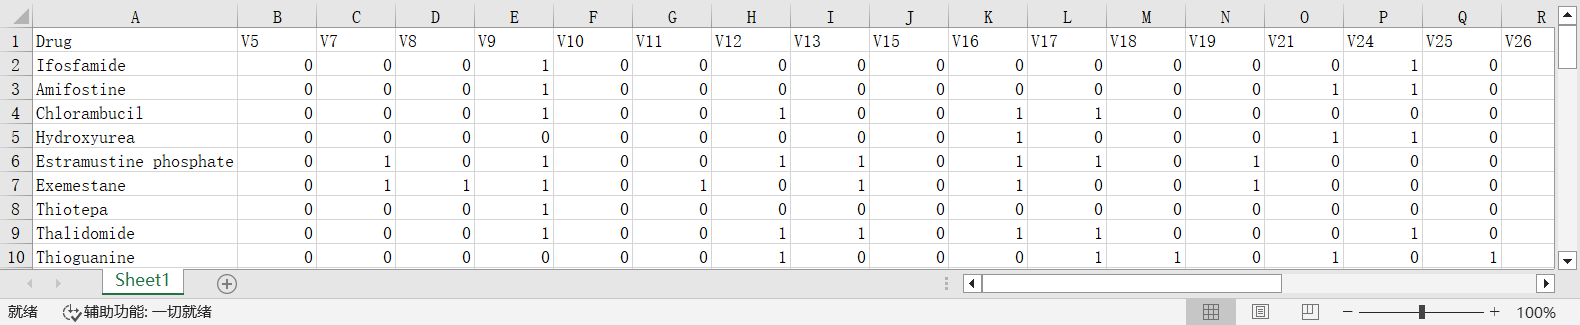
\includegraphics[width=0.8\textwidth]{3}
% \caption{文件50种药物分子指纹.xlsx的部分数据展示\label{fig:ndd}}
% \end{figure}

\begin{table}[htbp]
\centering
\caption{NCI-ALMANAC数据集药物分子指纹的部分数据展示\label{tb:ndd}}
\small
\begin{tabular}{p{2.5cm} p{1.2cm} p{1.2cm} p{1.2cm} p{1.2cm} p{1.2cm} p{1.2cm} p{1.2cm}}
\toprule
Drug & V5 & V7 & V8 & V9 & V10 & V11 & ... \\
\midrule
Ifosfamide & 0 & 0 & 0 & 1 & 0 & 0 & ... \\
Amifostine & 0 & 0 & 0 & 1 & 0 & 0 & ... \\
Chlorambucil & 0 & 0 & 0 & 1 & 0 & 0 & ... \\
Hydroxyurea & 0 & 0 & 0 & 0 & 0 & 0 & ... \\
% Estramustine phosphate sodium & 0 & 1 & 0 & 1 & 0 & 0 & ... \\
% Exemestane & 0 & 1 & 1 & 1 & 0 & 1 & ... \\
% Thiotepa & 0 & 0 & 0 & 1 & 0 & 0 & ... \\
... & ... & ... & ... & ... & ... & ... & ... \\
\bottomrule
\end{tabular}
\end{table}

\begin{table}[htbp]
\centering
\caption{NCI-ALMANAC数据集协同得分的部分数据展示\label{tb:ns}}
\small
\begin{tabular}{p{2.5cm} p{2.5cm} p{1.4cm} p{1.4cm} p{1.4cm} p{1.4cm} p{0.5cm}}
\toprule
DrugA & DrugB & 786-0 & A498 & A549 & ACHN & ... \\
\midrule
Ifosfamide & Chlorambucil & -277.60 & -266.71 & -245.81 & -240.25 & ... \\
Amifostine & Ifosfamide & -323.37 & -310.81 & -286.64 & -281.03 & ... \\
Amifostine & Chlorambucil & -176.69 & -259.98 & -267.98 & -209.61 & ... \\
Chlorambucil & Exemestane & -98.88 & -182.90 & -179.01 & -177.18 & ... \\
% Hydroxyurea & Chlorambucil & -217.29 & -269.98 & -228.54 & -136.28 & ... \\
... & ... & ... & ... & ... & ... & ... \\
\bottomrule
\end{tabular}
\end{table}

% \begin{figure}[htbp!]
% \centering
% 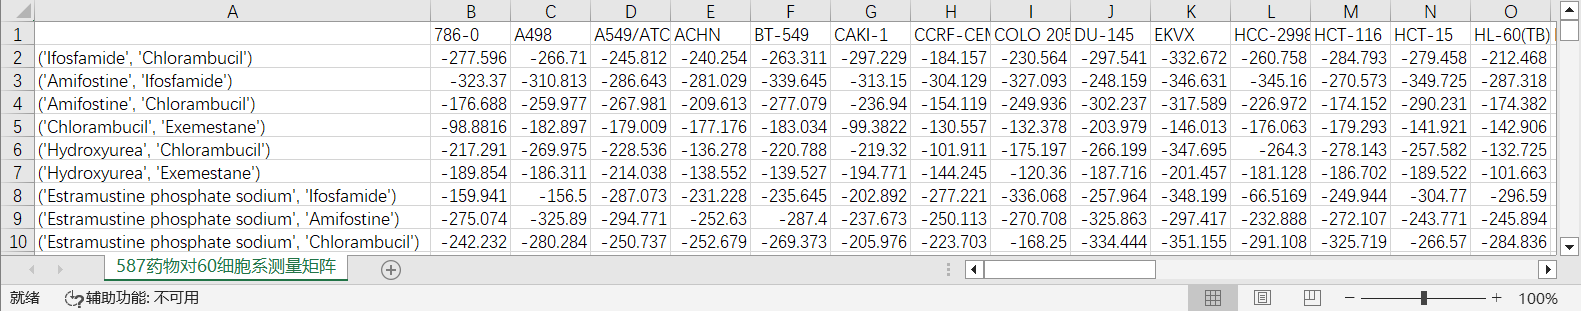
\includegraphics[width=0.8\textwidth]{4}
% \caption{文件587药物组合60细胞系测量矩阵.csv的部分数据展示\label{fig:ns}}
% \end{figure}

\section{数据预处理}

在类似于本文的相关研究中,通常使用原始数据进行模型的构建和求解。例如,岭回归方法要求目标矩阵的核范数最小并且接近原始矩阵,因此无需对原始数据进行标准化处理。而随机森林则是一种基于决策树的集成学习方法,它可以通过随机选择子样本和特征来构建多个决策树,并使用这些决策树的预测结果进行集成。由于随机森林是基于树的模型,不会受到数据缩放的影响,因此也无需对原始数据进行标准化处理。

\begin{figure}
\centering
  \begin{minipage}{0.45\linewidth}
    \centering
    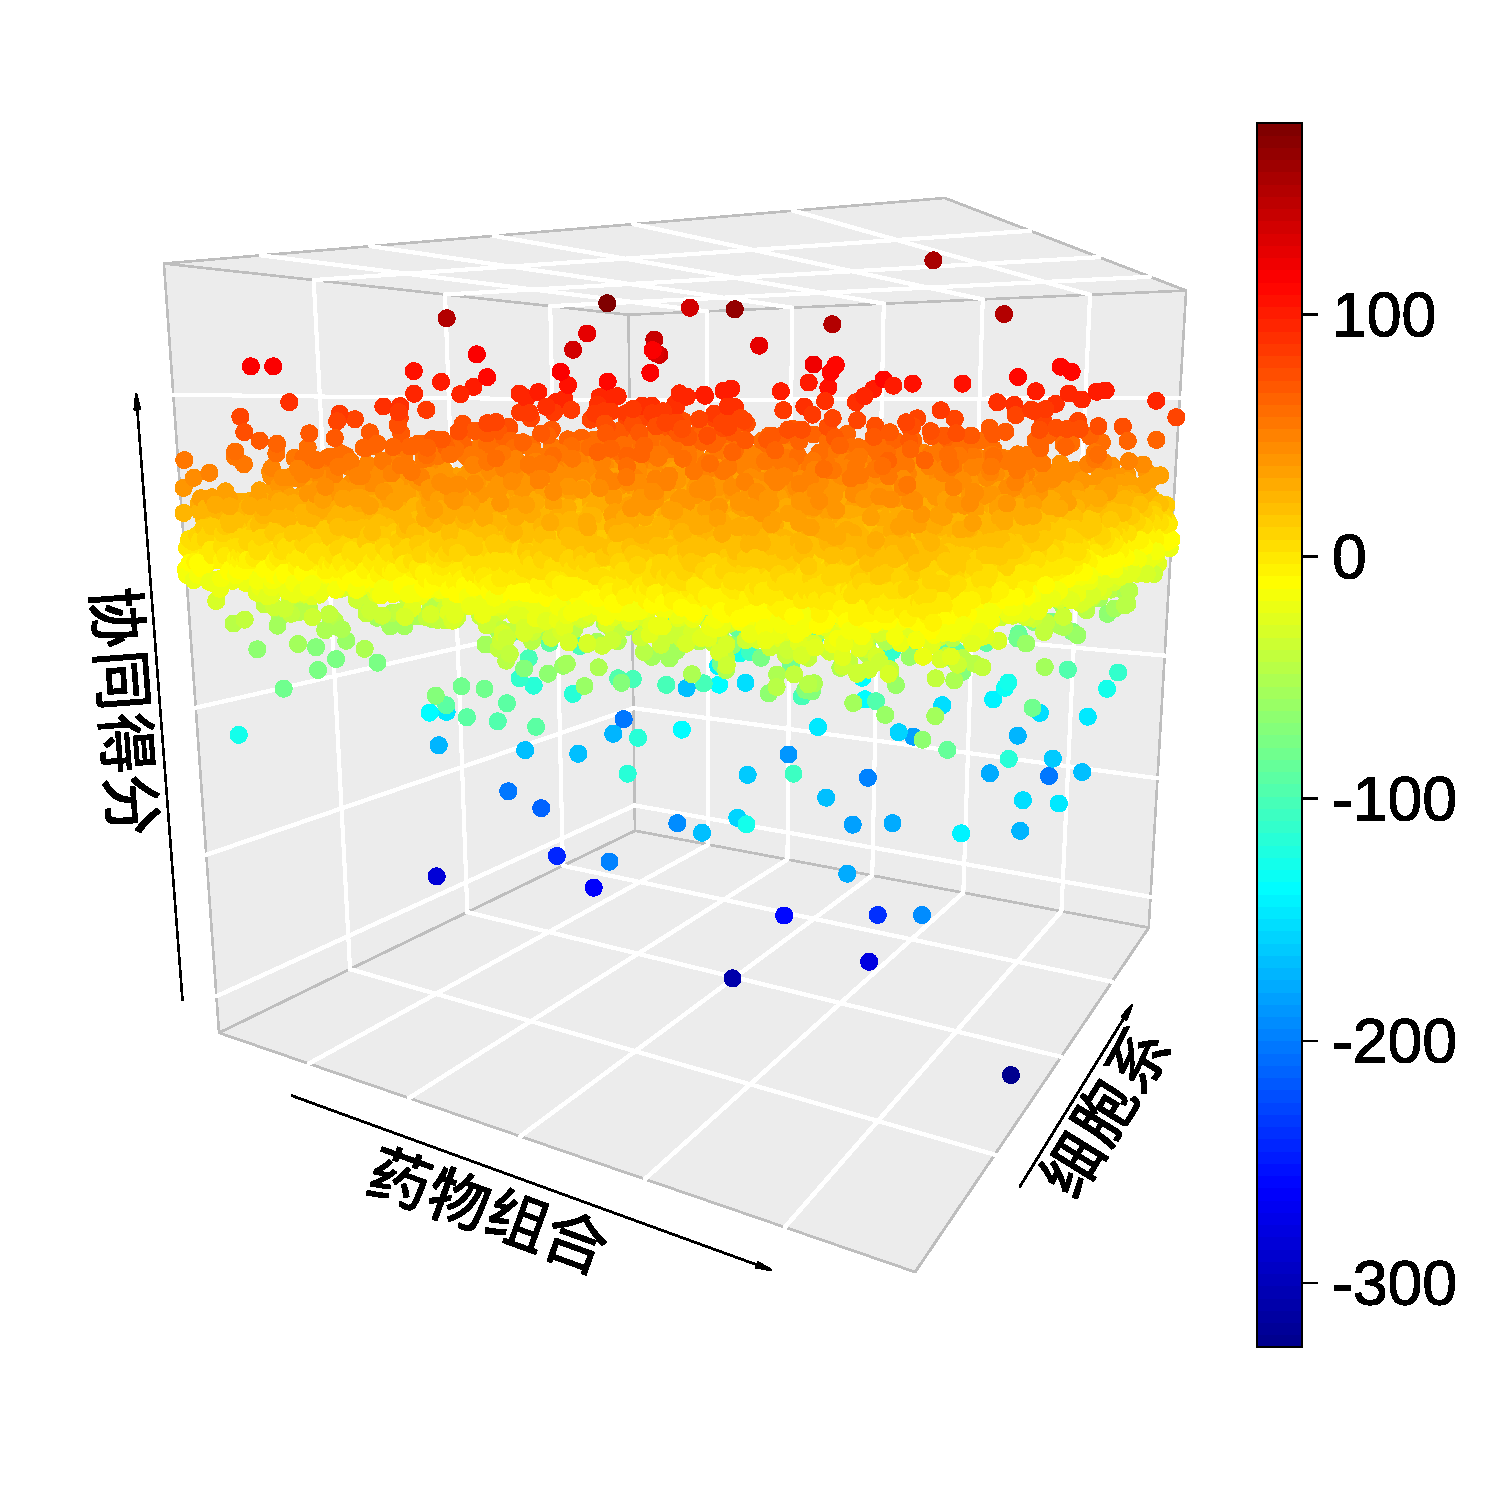
\includegraphics[width=\linewidth]{figures/old_o.pdf}
    \caption{基于O'Neil数据集\\协同得分的原始数据分布}
    \label{fig:sub1}
  \end{minipage}%
  \begin{minipage}{0.45\linewidth}
    \centering
    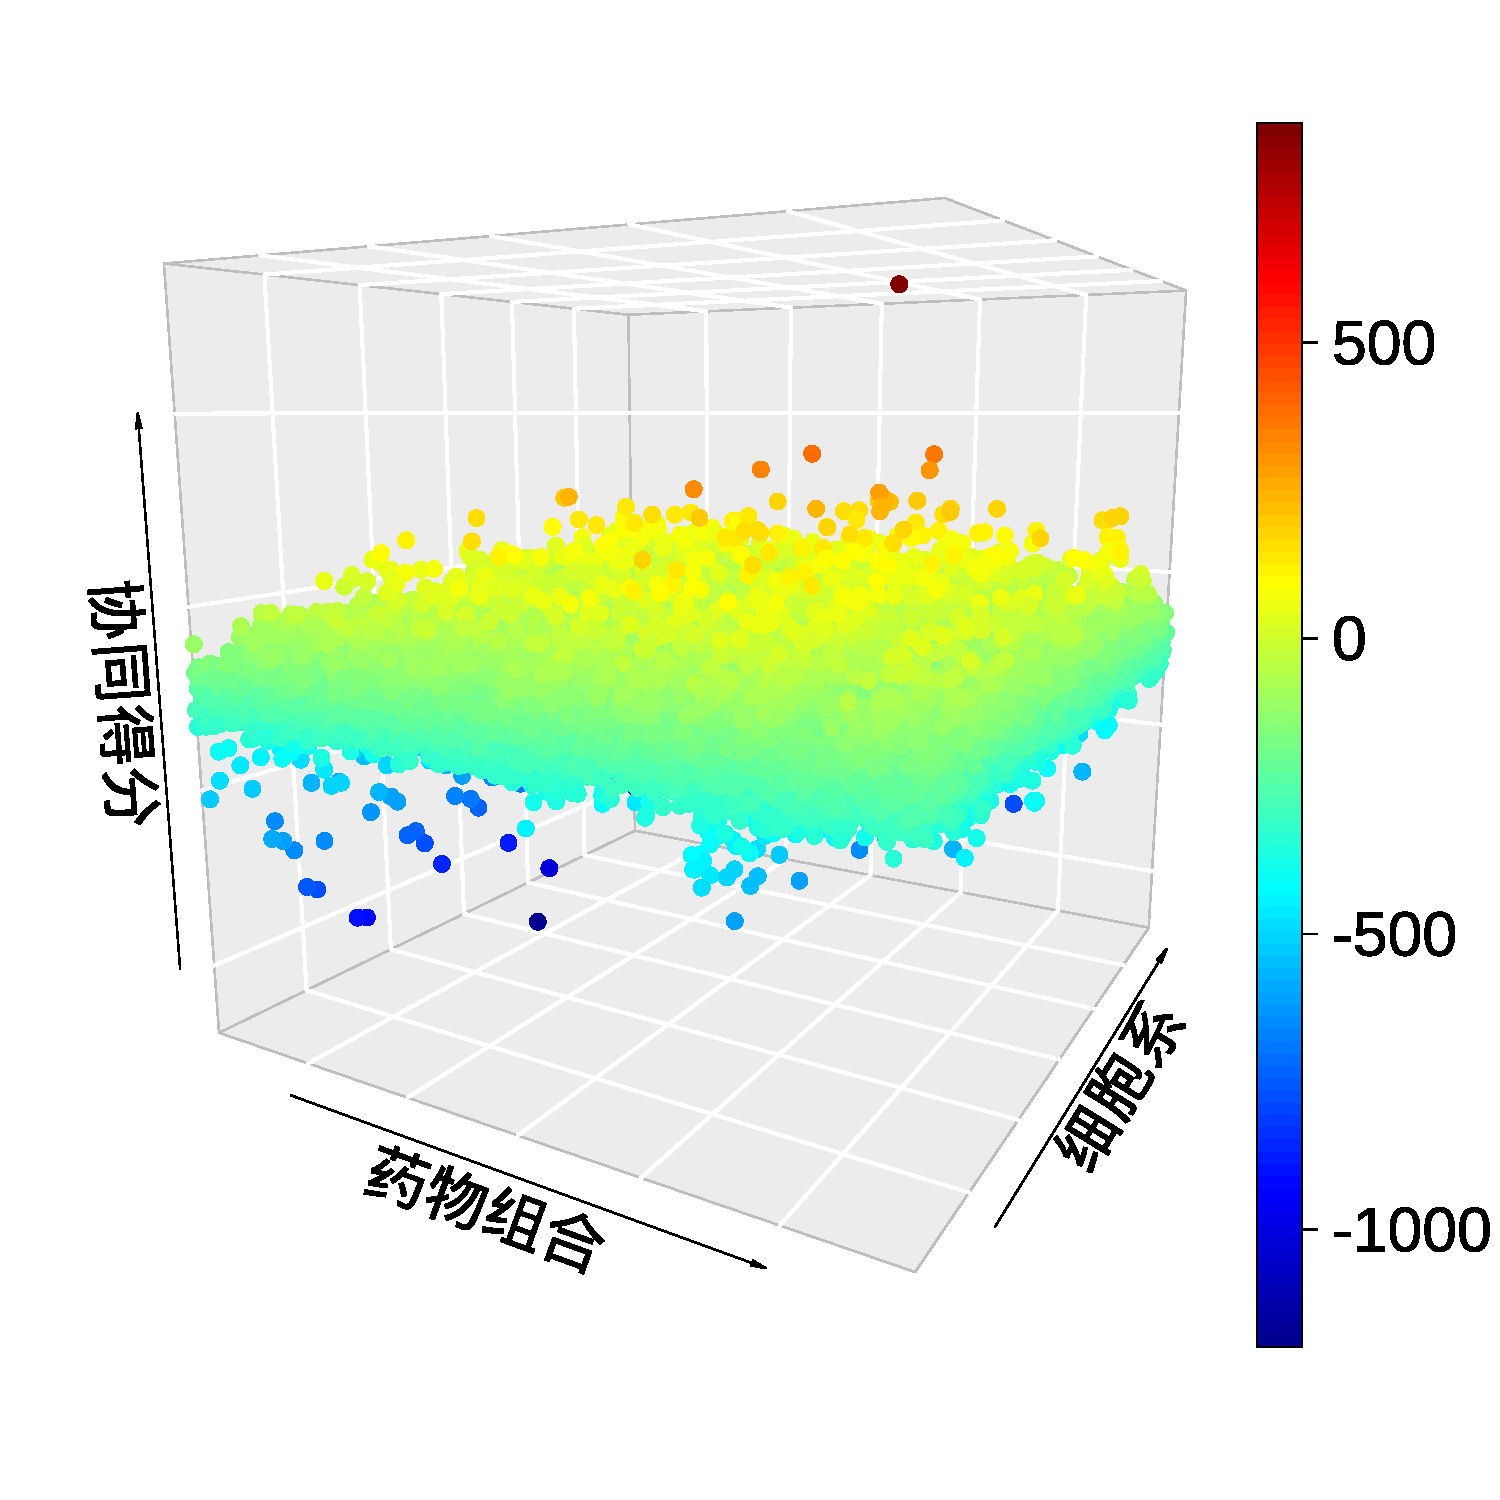
\includegraphics[width=\linewidth]{figures/new_o.pdf}
    \caption{基于NCI-ALMANAC数据集\\协同得分的原始数据分布}
    \label{fig:sub3}
  \end{minipage}
\end{figure}

本文需要使用基于高斯核函数扩展的权重函数来预测各目标药物组合的协同得分,需要使用高相似的药物组合的协同得分来预测目标药物组合的协同得分。图~\ref{fig:sub1}和图~\ref{fig:sub3}展示了本文的原始数据集中的协同得分部分,经过观察,可以发现在原始数据集中,大部分数据都分布在中间范围内,但同时也存在一些数据的测量结果明显偏大或偏小,分布不均匀有极端值。当原始数据的差异较大时,部分高相似的药物组合的权重会过高,从而影响预测结果。因此,在使用前需要对原始数据进行标准化处理\supercite{20}。

本文对两个数据集中的协同得分进行了Z-score行标准化处理,让标准化后的数据具有相同的均值和标准差,以使得不同药物组合之间的值具有可比性,方便数据的比较和分析。如果不进行Z-score行标准化处理,部分数据的数值差异过大,也会影响到后续的相似性系数计算结果。在计算Tanimoto相关系数时,奇异值可能会影响排名的计算,从而影响系数的计算结果。在计算Spearman相关系数时,数据集中存在极端值或异常值可能会导致计算得到的排名与实际情况不符,从而影响计算结果。

\begin{equation}
z_{ij} = \frac{x_{ij} - \mu_j}{\sigma_j}.
\end{equation}

\noindent 其中,$x_{ij}$ 是第 $i$ 行第 $j$ 列的数据,$\mu_j$ 是第 $j$ 列的均值,$\sigma_j$ 是第 $j$ 列的标准差,$z_{ij}$ 是标准化后的第 $i$ 行第 $j$ 列的值。对于每一列数据,先计算出其均值 $\mu_j$ 和标准差 $\sigma_j$,然后用上述公式将每一行的数据进行标准化。标准化后的数据满足均值为0,标准差为1的正态分布。

\newpage

\begin{figure}
\centering
  \begin{minipage}{0.45\linewidth}
    \centering
    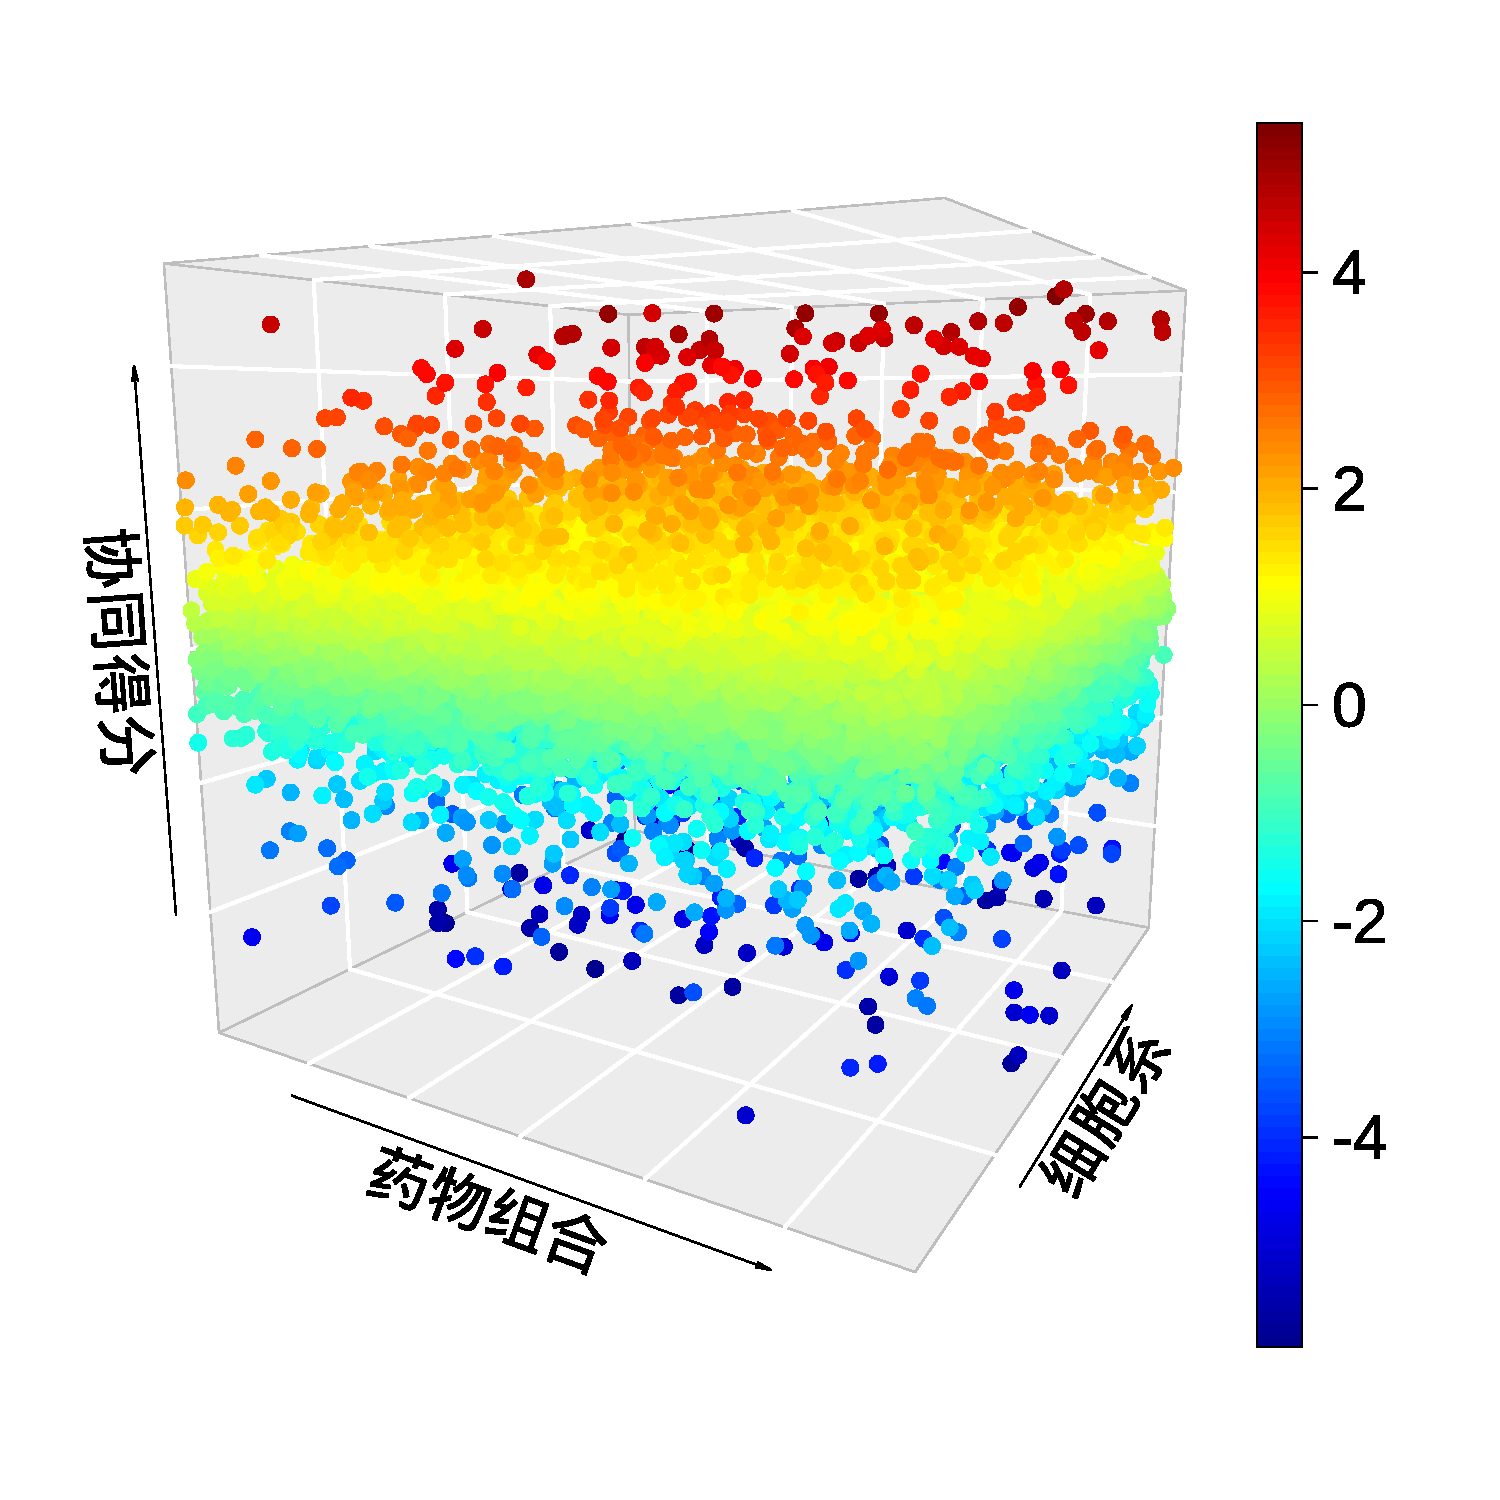
\includegraphics[width=\linewidth]{figures/old_n.pdf}
    \caption{基于O'Neil数据集\\协同得分标准化后的数据分布}
    \label{fig:sub2}
  \end{minipage}%
  \begin{minipage}{0.45\linewidth}
    \centering
    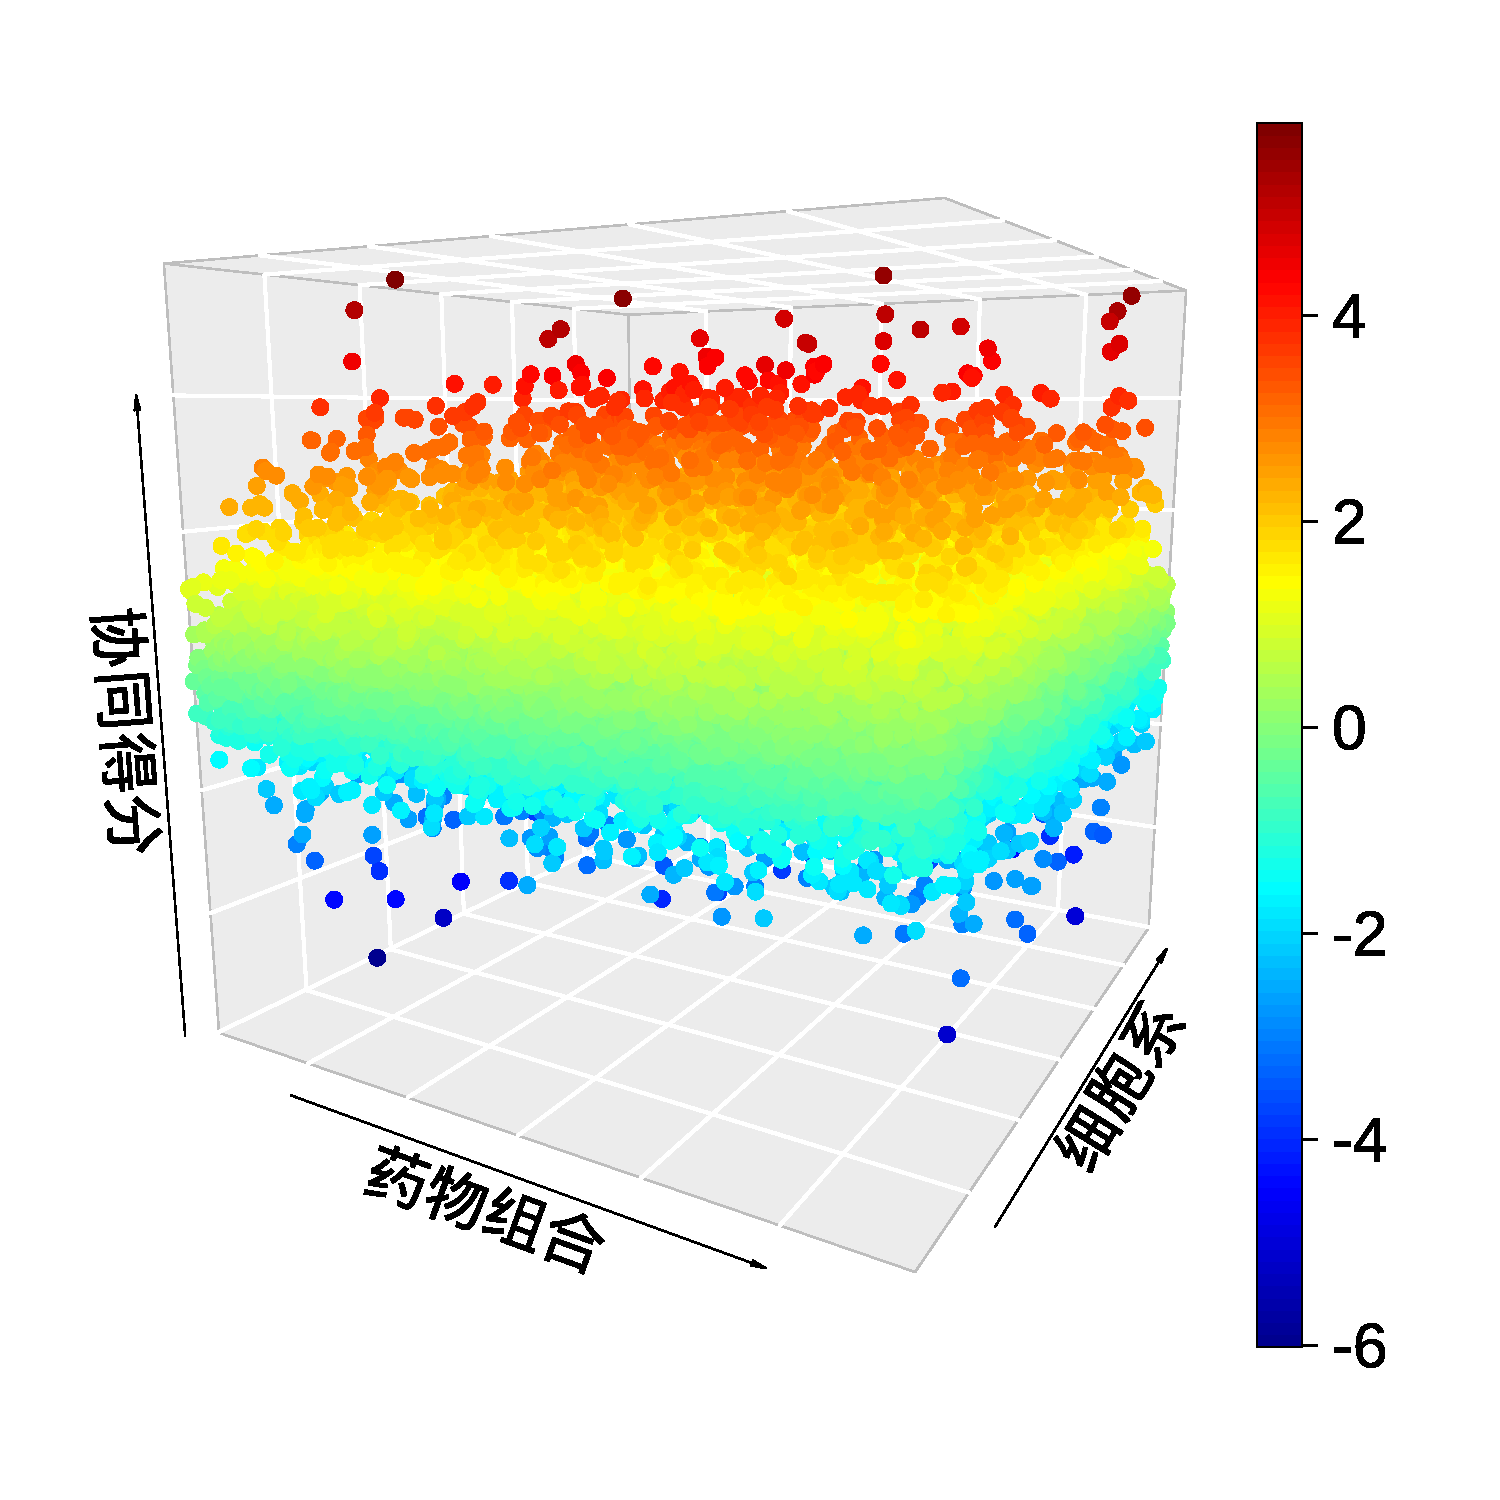
\includegraphics[width=\linewidth]{figures/new_n.pdf}
    \caption{基于NCI-ALMANAC数据集\\协同得分标准化后的数据分布}
    \label{fig:sub4}
  \end{minipage}
\end{figure}

图~\ref{fig:sub2}和图~\ref{fig:sub4}展示了本文的标准化后数据集中的协同得分部分。对于经过预处理的数据集,由于经过了标准化处理,数据分布变得更加均匀了,这表明数据已经成功地去除了初始的偏差。使用预处理后的数据进行后续的模型构建和求解,将不再出现因某一药物权重过高而导致模型偏差的现象,模型的预测效果更为准确。

\section{本章小结}

本章主要介绍了前期工作中所采用的数据集和数据预处理方法。研究使用了O'Neil数据集和NCI-ALMANAC数据集进行实验,以验证提出的模型在不同数据集上的泛化能力和有效性。数据集的处理包括对O'Neil数据集和NCI-ALMANAC数据集中的协同得分进行Z-score行标准化处理,以确保数据具有可比性和一致性。这些处理能够提高模型的性能和准确度,并深入研究这些数据集的特性和规律。
  % !Mode:: "TeX:UTF-8"
\chapter{基于药物组合相似性网络的模型构建与求解}
\label{chap:theory}

\section{药物组合相似性假设及其验证}

\subsection{药物组合相似性计算}

本文使用药物分子指纹构建药物组合分子指纹,再使用药物组合分子指纹计算药物组合的相似系数。分子指纹是用于描述化合物结构的一种有效方法。该方法通过检测药物分子结构中的一些特定子结构是否存在,例如原子、键和环等,将分子结构转化为一系列0-1序列,从而对药物化合物的结构和性质进行编码和比较。这是一种快速、高效的结构描述工具,可用于计算化学、药物研究和分子设计等领域。由于药物分子指纹可以快速计算和比较,因此被广泛应用于虚拟筛选、化学信息学和计算化学等领域\supercite{21}。本文假设$d_i$表示药物$i$的分子指纹序列,$d_j$表示药物$j$的分子指纹序列:

\vspace{-1.5em}

\begin{equation*}
d_i = (d_{i1}, d_{i2}, \ldots, d_{in}),
\end{equation*}

\vspace{-1.5em}

\begin{equation*}
d_j = (d_{j1}, d_{j2}, \ldots, d_{in}),
\end{equation*}

\noindent 药物$d_i$和药物$d_j$横向拼接分子指纹序列获得药物组合$D$的分子指纹序列,即$D$表示为:

\vspace{-1.5em}

\begin{equation*}
\large D=(d_i, d_j) \text{ 或 } D=(d_j, d_i).
\end{equation*}

为了量化药物组合间的相似性,本文基于药物的分子指纹使用Tanimoto系数\supercite{23}计算药物组合的相似系数。Tanimoto系数是一种衡量两个分子之间相似程度的量化指标,当Tanimoto系数越高时,代表着两个分子的结构越相似。这种相似性可能意味着它们具有类似的生物活性、药理作用、代谢途径等。Tanimoto系数是一种广泛应用于化学结构相似性评估的指标,特别适用于评估分子之间的相似性。该系数的计算结果介于0和1之间,其中1表示两个分子完全相同,而0表示两个分子没有共同特征。根据该系数的定义,药物组合的Tanimoto系数矩阵如式(\ref{eq:dm}):

\vspace{-1em}

\begin{equation}
\mathbfit{T} = (T_{ij})_{m\times n},\label{eq:dm}
\end{equation}

\noindent 其中

\begin{equation}
T_{ij} = T(D_i, D_j) = \frac{|D_i \cap D_j|}{|D_i \cup D_j|},\label{eq:T}
\end{equation}

\noindent $m$为药物组合的个数,$D_i$和$D_j$分别为药物组合$i$和药物组合$j$。

在实际计算药物组合的Tanimoto系数时,需要考虑药物组合$D_i$和药物组合$D_j$之间的顺序以及它们自身分子指纹中单药横向拼接的顺序。这些顺序对计算结果都有影响,可能导致不同的结果。因此,在进行计算时,需要遍历四个不同的排列顺序,包括$D_i$和$D_j$之间的顺序以及它们自身分子指纹的顺序,然后选择最大值作为$D_i$和$D_j$之间的Tanimoto系数。通过这种方式,可以获得更准确、更可靠的结果。

\subsection{相似性假设的提出}

2015年,张乃千等人发现了“基因组信息相似的细胞系和分子结构相似的药物对应的药物反应谱更为相似”这一现象,构建了细胞系-药物双层网络模型,与局部线性方法相结合预测抗癌药物对于细胞系的敏感性,取得了较好的效果\supercite{15}。受此启发,本文拟通过药物组合-细胞系的协同得分构建DCSN模型。此时,在给定一个固定的细胞系的情况下,利用高相似药物组合的协同得分可以预测目标药物组合的协同得分。这种方式能够充分利用已有的相似药物组合信息,为预测目标药物组合的协同得分提供参考依据。DCSN模型的前提假设是“相似药物组合对固定细胞系具有相似的协同作用”。只有在该前提成立的情况下,模型才能有效进行预测,接下来本文将对该假设进行验证。

\subsection{相似性假设的验证}

\textbf{相似性阈值设置的可行性}

本文使用O'Neil数据集和NCI-ALMANAC数据集,分别计算了每个数据集药物组合之间的Tanimoto系数。由于Tanimoto系数矩阵数据量较大,因此本文采用了t-SNE降维方法(如式(\ref{eq:t1})、式(\ref{eq:t2})、式(\ref{eq:t3})),将数据降维到三维,以探索是否存在相似性关系\supercite{29}。t-SNE的核心思想是将高维空间中距离近的点映射到低维空间中距离仍然近的点,而将距离远的点映射到距离更远的点,以保留原始数据中的局部结构信息。通过最小化cost函数,t-SNE优化低维嵌入,使得低维空间中相似度与高维空间中相似度相近,从而实现数据降维与可视化。这一方法可以用于探索数据是否存在内在结构和规律。因此,本文采用了t-SNE方法,将高维的Tanimoto系数矩阵数据降维到三维,以便于观察和分析数据之间的相似性关系。

\begin{equation}
p_{ij} = \frac{\exp(-\lVert x_i - x_j \rVert^2 / 2\sigma^2)}{\sum_{k \neq l} \exp(-\lVert x_k - x_l \rVert^2 / 2\sigma^2)},\label{eq:t1}
\end{equation}

\begin{equation}
q_{ij} = \frac{(1 + \lVert y_i - y_j \rVert^2)^{-1}}{\sum_{k \neq l} (1 + \lVert y_k - y_l \rVert^2)^{-1}},\label{eq:t2}
\end{equation}

\begin{equation}
C = KL(P || Q) = \sum_i \sum_j p_{ij} \log \frac{p_{ij}}{q_{ij}}.\label{eq:t3}
\end{equation}

\noindent 其中,$p_{ij}$ 表示在高维空间中点 $x_i$ 与点 $x_j$ 的相似度,由高斯分布计算而得,分母为归一化系数;$q_{ij}$ 表示在低维空间中点 $y_i$ 与点 $y_j$ 的相似度,由t分布计算而得,分母为归一化系数;$KL$ 表示KL散度,用于度量两个概率分布之间的距离;$C$ 表示 cost 函数,用于评估低维空间与高维空间的相似度。

在t-SNE降维的实现过程中,需要注意Tanimoto系数矩阵是一个沿主对角线对称的矩阵,其中主对角线上的系数对应每种药物组合自身的相关系数全为1。因此,需要将矩阵的下三角元素赋值为0,并且只使用矩阵的上三角数据进行计算。t-SNE是基于相似度或距离矩阵进行降维的,只要相似度或距离矩阵保持不变,那么降维的结果也不会发生变化。将下三角数据设置为0相当于将这些数据作为距离矩阵的缺失值处理,不会对上三角数据的权重产生影响,从而不会对t-SNE的结果产生影响。具体而言,通过t-SNE将数据降至三维,并将其制作成三维散点图,如图\ref{fig:mts}和图\ref{fig:nts}所示。

\begin{figure}[H]
\centering
  \begin{minipage}{0.5\linewidth}
    \centering
    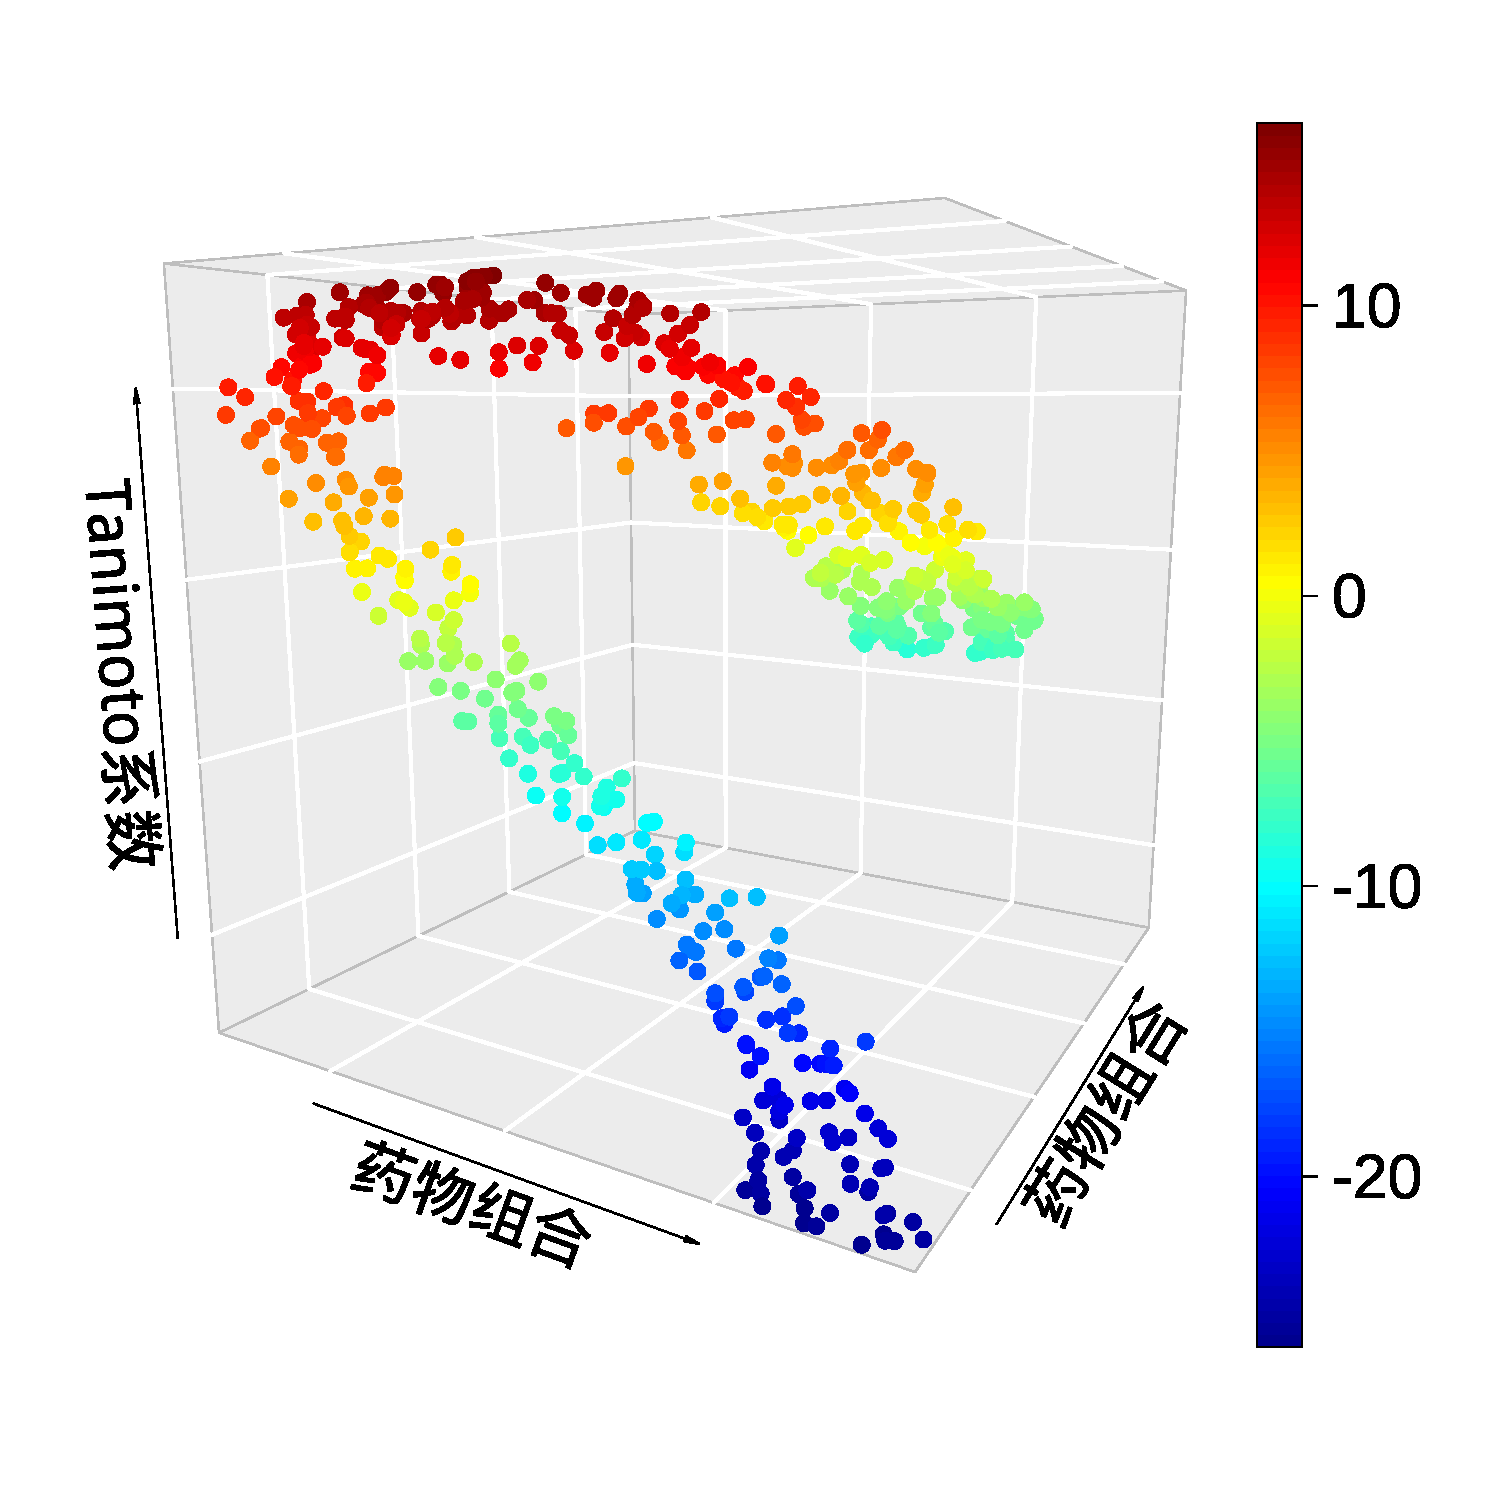
\includegraphics[width=\linewidth]{figures/o_t_sne.pdf}
    \caption{基于t-SNE的O'Neil数据集\\Tanimoto系数散点图}\label{fig:mts}
  \end{minipage}%
  \begin{minipage}{0.5\linewidth}
    \centering
    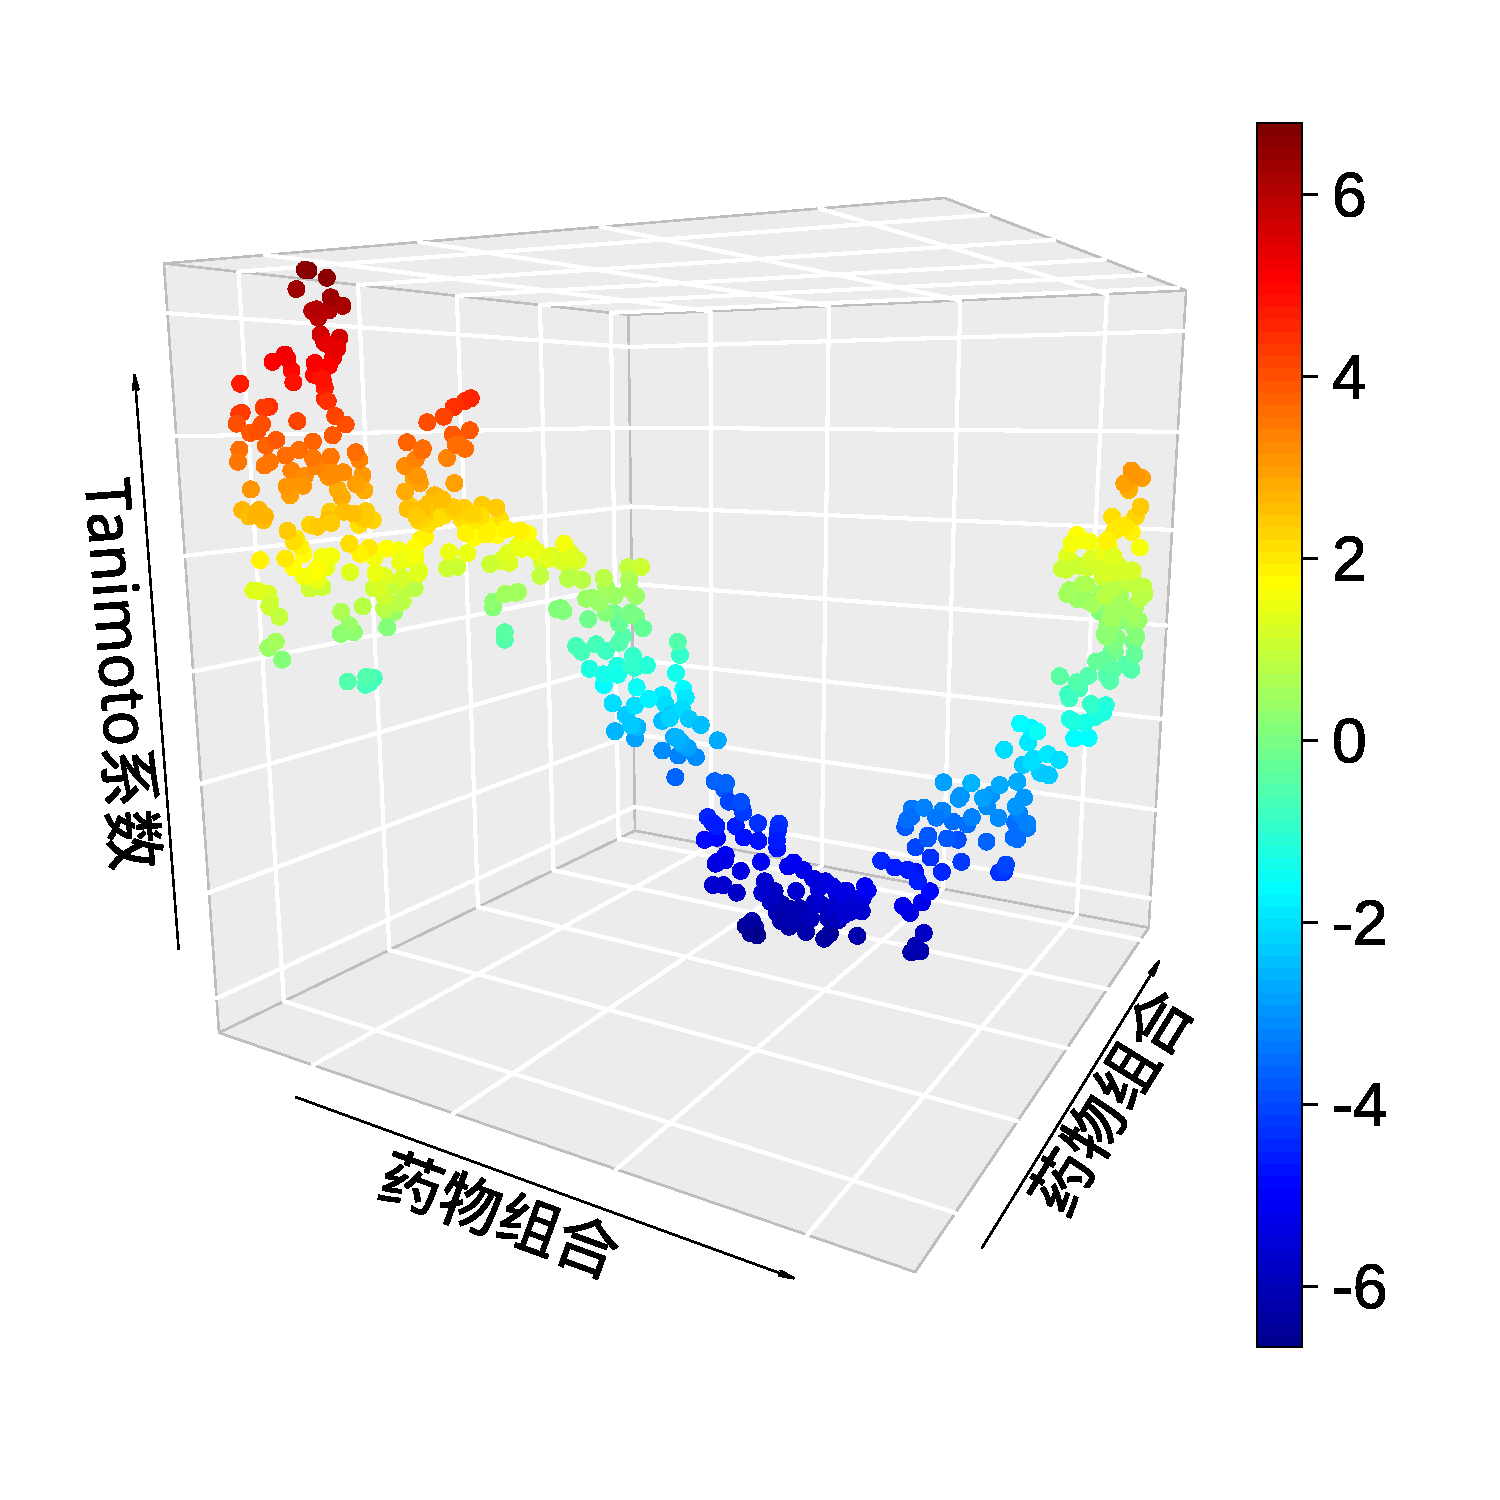
\includegraphics[width=\linewidth]{figures/n_t_sne.pdf}
    \caption{基于t-SNE的NCI-ALMANAC数据集\\Tanimoto系数散点图}\label{fig:nts}
  \end{minipage}
\end{figure}

观察三维散点图,无论使用哪个数据集,散点都呈现出一种类似于跨越整个三维空间的对角线簇的趋势。这暗示了数据集本身具有一定的内在结构,可以使用低维空间中的一条曲线簇来进行近似表示。这也表明,数据集中存在着某种相似性和规律性,这些特征可以通过降维后的曲线簇来进行表示。本文则认为,不同的数据点可能具有相似的特征或属性,因此它们在低维空间中会聚集成曲线簇。在高维空间中,数据点之间存在某种程度的相似性或相关性,而这种相似性或相关性在低维空间中被保留下来。同时,在低维空间中,数据点之间的距离关系也得到了保留。相距较远的点在三维空间中仍然相距较远,而相距较近的点在三维空间中也比较接近。这说明t-SNE算法可以在保留数据局部结构的同时,尽可能地减少不同类别之间的干扰。

\vspace{-1em}

\begin{equation}
\mathbfit{Hd} = \begin{bmatrix} T_1^{(1)} \\ \vdots \\ T_n^{(1)} \end{bmatrix}, \qquad 
\mathbfit{Ld} = \begin{bmatrix} T_1^{(2)} \\ \vdots \\ T_n^{(2)} \end{bmatrix}.
\label{eq:hdld}
\end{equation}

基于以上分析,本文认为可以利用Tanimoto系数并设置相似性系数的阈值来对数据集进行划分,以识别高相似性药物组合团和低相似性药物组合团。这种方法有助于进一步挖掘数据集中的相似性和规律性,以更好地理解数据集中的特征和属性。在前文提到的三维散点图中,可以通过在两个水平方向上进行横截面分割,将散点分成相应的高\texttt{\symbol{92}}低相似药物组合散点团。根据这些药物组合团的名称,可以将药物组合-细胞系的协同得分矩阵分成两个矩阵(\ref{eq:hdld})。具体而言,即根据式(\ref{eq:dm})和式(\ref{eq:T})计算的结果,药物组合可以分为两个团体,其中Tanimoto系数大于$α$的药物组合属于高相似药物组合团$\mathbfit{Hd}$,而Tanimoto系数小于$β$的药物组合则属于低相似药物组合团$\mathbfit{Ld}$。

\textbf{基于相似性阈值的协同得分分布}

假设药物组合个数为$m$,细胞系个数为$n$,药物组合$D_i$与细胞系$C_j$之间的协同得分表示为$S_{ij}$,药物组合-细胞系的协同得分矩阵表示为

\vspace{-1em}

\begin{equation}
\mathbfit{S} = (S_{ij})_{m\times n},
\end{equation}

\noindent 分别对$\mathbfit{Hd}$和$\mathbfit{Ld}$中对应的$S_i^{(1)}, S_i^{(2)}$进行Spearman相关系数的计算,如

% \vspace{-1em}

\begin{equation}
r_i^k=1-\frac{6\sum_{i=1}^n(S_i^{(k)}-S_i^{(k)})^2}{n(n^2-1)} \quad (k=1 \text{ 或 } k=2).
\label{eq:sp}
\end{equation}

这里在考察药物组合团的协同作用时,使用了Spearman相关系数\supercite{24}来度量最终高相似与低相似药物组合团的协同作用。Spearman相关系数可用于评估不同药物组合相似性和它们在协同作用方面的表现是否相似。具体而言,当两种药物组合的相似性越高时,如果它们在协同作用方面的表现也越相似,则它们的Spearman相关系数会更高;反之,当两种药物组合的相似性越低时,它们在协同作用方面的表现如果越不相似,则它们的Spearman相关系数会更低。高相似药物组合-细胞系协同得分的Spearman相关系数矩阵$\mathbfit{M_1}$和低相似药物组合-细胞系协同协同得分的Spearman相关系数矩阵$\mathbfit{M_2}$:

\vspace{-1em}

\begin{equation*}
\mathbfit{M_1} = \begin{pmatrix} r_1^{(1)} & r_2^{(1)} & \cdots & r_n^{(1)} \end{pmatrix}, 
\end{equation*}

\vspace{-1em}

\begin{equation*}
\mathbfit{M_2} = \begin{pmatrix} r_1^{(2)} & r_2^{(2)} & \cdots & r_n^{(2)} \end{pmatrix}.
\end{equation*}

基于O'Neil数据集的实验结果显示,当Tanimoto系数的临界值$α$被设定为0.60,临界值$β$被设定为0.52时,高低相似药物组合的数量近似相同,其中高相似性药物组合的数量为11个,低相似药物组合的数量为13个。针对这些数据,可以绘制两个药物组合团相关性分布的箱线图,如图\ref{fig:1g}所示。同时,基于NCI-ALMANAC数据集的实验结果显示,当Tanimoto系数的临界值$α$被设定为0.55,临界值$β$被设定为0.52时,高相似药物组合和低相似药物组合的数量近似相同。其中,高相似性药物组合的数量为38个,而低相似药物组合的数量为35个。根据这些数据,可以绘制两个药物组合团相关性分布的箱线图,如图\ref{fig:2g}所示。

\begin{figure}[H]
\centering
  \begin{minipage}{0.45\linewidth}
    \centering
    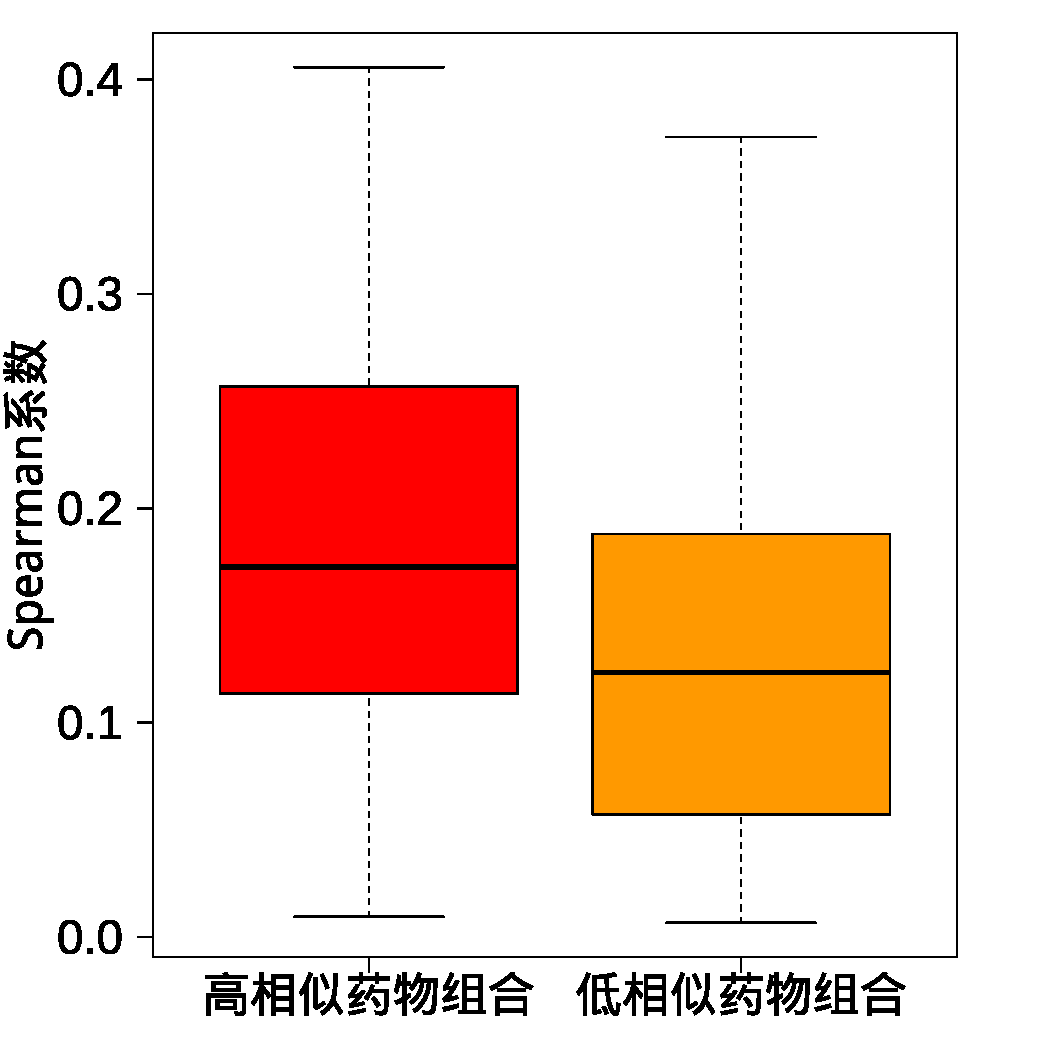
\includegraphics[width=\textwidth]{figures/O箱线图.pdf}
    \caption{O'Neil数据集\\药物组合相似性假设验证\label{fig:1g}}
  \end{minipage}%
  \begin{minipage}{0.45\linewidth}
    \centering
    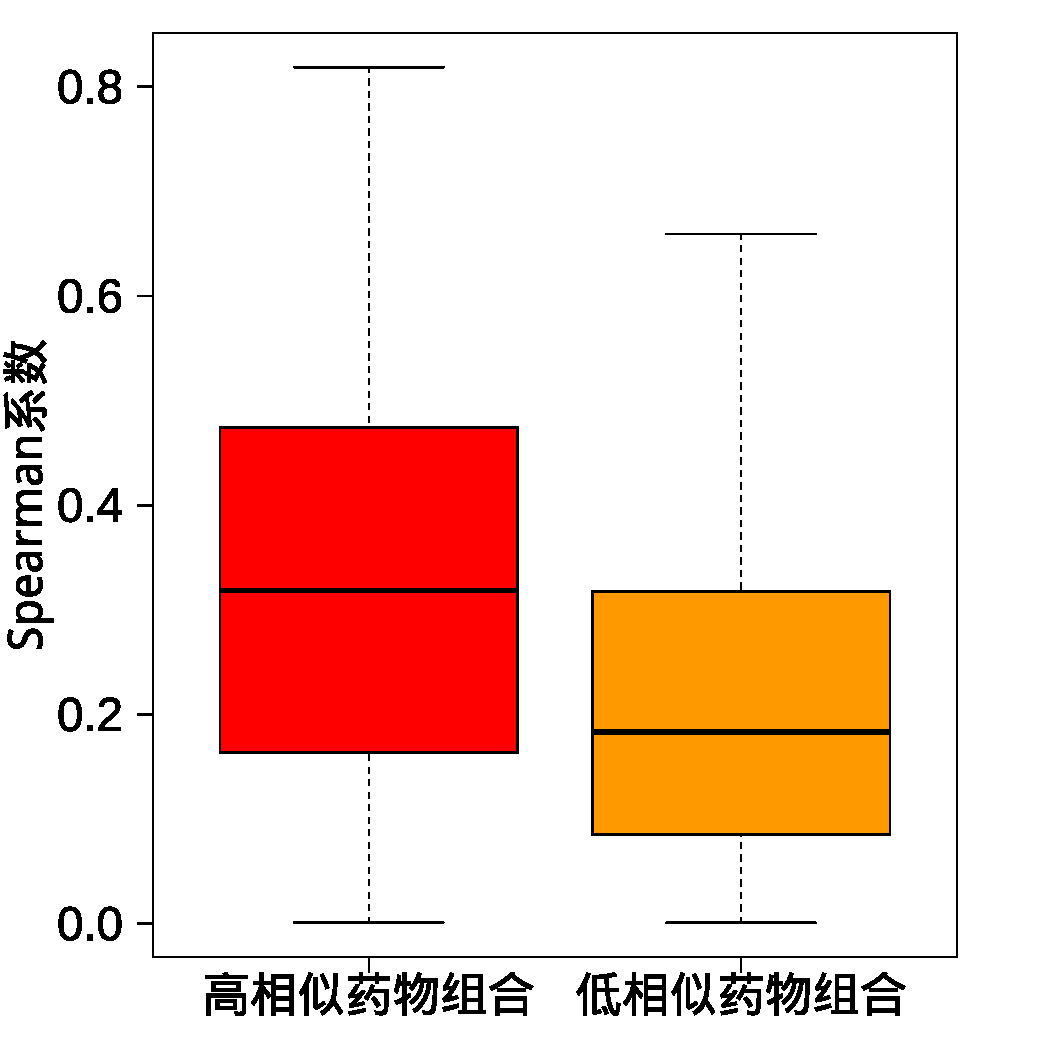
\includegraphics[width=\textwidth]{figures/NCI箱线图.pdf}
    \caption{NCI-ALMANAC数据集\\药物组合相似性假设验证\label{fig:2g}}
  \end{minipage}
\end{figure}

\vspace{-1em}

通过图\ref{fig:1g}和图\ref{fig:2g}可以更加清晰地了解高相似性药物组合和低相似药物组合之间的差异和共性。显然,高相似药物组合协同得分的Spearman相关系数明显高于低相似药物组合的Spearman相关系数,“相似药物组合对固定细胞系具有相似的协同作用”的假设验证成立,模型构建的前提条件成立。在此前提下,构建模型可以使用高相似药物组合去预测目标药物组合的协同作用。

\section{药物组合相似性网络模型的构建}

参考文献\cite{15}中基于药物相似性网络构建的单层网络预测模型中,认为与药物$D$化学结构相似性高的药物$D_j$与细胞系$C$的药物敏感性相比于其它药物与细胞系$C$的药物敏感性对模型的预测有更高的贡献。因此,该文献的模型给与药物$D$具有高相似的药物$D_j$对于细胞系$C$的药物敏感性以更高的权重,给与药物$D$具有低相似的药物对于细胞系$C$的药物敏感性以更低的权重,这里的权重函数$\omega(D,D_j)$是药物$D_j$与药物$D$的相关系数的单增函数,具体形式为:

\begin{equation}
\omega(D,D_j)=\exp\left(-\frac{[1-\rho(D,D_j)]^2}{2\tau^2}\right).\label{eq:znc}
\end{equation}

该权重函数$\omega(C,C_i)$基于高斯核函数$w(x_i, x_j)$扩展而来的。在许多ML方法中,经常需要定义一种权重函数来衡量不同样本之间的相似度或距离。高斯核函数是一种常用的权重函数,它以高斯(正态)分布的形式将权重分布在样本周围,其定义如下:

\vspace{-1em}

\begin{equation*}
w(x_i, x_j) = \exp\left(-\frac{{\|x_i - x_j\|^2}}{{2\sigma^2}}\right).
\end{equation*}

\noindent 其中,$w(x_i, x_j)$表示样本$x_i$和$x_j$之间的权重,$|x_i - x_j|$表示欧氏距离,$\sigma$表示高斯核函数的带宽(控制权重函数的宽窄程度)。在实际应用中,通常需要根据具体问题和数据的特点来选择适当的带宽参数$\sigma$。较小的$\sigma$会使得权重函数在样本周围的区域变得更加尖锐,更加注重局部相似性;而较大的$\sigma$会使得权重函数在整个样本空间内分布更均匀,更加注重全局相似性。

本文借鉴了药物敏感性预测的局部加权模型(\ref{eq:znc}),类似的提出了药物组合相似性网络模型(DCSN)的权重函数(\ref{eq:omg}):

\begin{equation}
\omega(D,D_j)=\exp\left(-\frac{[1-T(D,D_j)]^2}{2\tau^2}\right).
\label{eq:omg}
\end{equation}

\noindent 其中,$T(D,D_j)$表示药物组合$D$和$D_j$的Tanimoto系数,$τ$表示药物组合相似性降低时的衰减率。本文认为与药物组合$D$相似性高的药物组合对细胞系的协同作用相比于其它相似性低的药物组合对细胞系的协同作用对模型的预测有更高的贡献。因此,DCSN模型给与药物组合$D$具有高相似的药物组合以更高的权重,给与药物组合$D$具有低相似的药物组合以更低的权重。

DCSN模型构建如下:

\begin{equation}
\hat{S}_1(D,C) = \frac{\sum\limits_{i=1}^N \omega(D,D_j) \mathbfit{S}(D_j,C)}{\sum\limits_{i=1}^N \omega(D,D_j)}.
\end{equation}

\noindent 其中,$ω(D,D_j)$表示通过权重函数(\ref{eq:omg})计算药物组合$D_j$对于$D$的权重,$\mathbfit{S}(D_j,C)$表示药物组合$D_j$对于细胞系$C$的协同得分测试值,$\hat{S}_1(D,C)$表示药物组合$D$对于细胞系$C$的协同得分预测值。在实验过程中,发现归一化的加权网络模型效果比未归一化的模型效果更好,在使用邻居药物组合去预测目标药物组合的协同作用得分时,在加权和${\sum\limits_{i=1}^N \omega(D,D_j) \mathbfit{S}(D_j,C)}$后除以了权重和${\sum\limits_{i=1}^N \omega(D,D_j)}$,使得模型的预测效果更优。

\section{模型求解}

本文使用留一交叉验证\cite{25}训练模型,确定模型参数,使用Pearson相关系数(PCC)评估模型的预测性能,具体操作过程如下:从所有的协同得分数据中取出一个药物组合数据作为测试集,剩余数据作为训练集,在此训练集之上建立模型,再在测试集上进行预测;数据集中每一个药物组合的数据都被逐一取出作为测试集,并用剩余的数据作训练集,建立模型求解,于是得到所有药物组合协同得分的预测值。测试集的药物组合不包含在训练数据中,这可以用来评估模型的泛化能力。

在药物组合相似性网络模型中,需要确定两个超参数,分别是药物组合高相似的邻居数$N$和药物组合相似性降低时的衰减率$τ$。其中,药物组合高相似的邻居数$N$是基于药物组合相似性指标Tanimoto系数确定的。因此,该参数可以由另一个超参数——药物组合的相似性阈值平替来确定。该阈值限制了药物组合高相似的药物组合邻居的Tanimoto系数大小。

在实际实验的过程中,考虑使用PCC最大和均方误差(MSE)最小作为目标进行求解,但考虑到相关模型使用原始数据进行预测和评价,而DCSN模型使用标准化后的数据进行预测和评价,不同模型横向比较MSE不具备实际意义,所以最终选择使用PCC最大作为目标函数求解。PCC的取值范围在$-1$到$+1$之间,其中$-1$表示完全的负相关,$+1$表示完全的正相关,$0$表示无相关性。PCC的计算基于两个变量之间的协方差和各自的标准差:

\begin{equation*}
\text{PCC} = \frac{\sum_{i=1}^{n}(x_i - \bar{x})(y_i - \bar{y})}{\sqrt{\sum_{i=1}^{n}(x_i - \bar{x})^2}\sqrt{\sum_{i=1}^{n}(y_i - \bar{y})^2}}.
\end{equation*}

\noindent 其中,$n$ 是样本数量,$x_i$ 和 $y_i$ 是第 $i$ 个样本的两个变量的取值,$\bar{x}$ 和 $\bar{y}$ 分别是两个变量的均值。PCC 的取值范围在 $[-1, 1]$,当 PCC 的值接近 1 时,表示两个变量正相关;当 PCC 的值接近 -1 时,表示两个变量负相关;当 PCC 的值接近 0 时,表示两个变量无线性相关关系。

因此,根据超参数的种类,可以得到四种有不同求解区间的方法,分别使用不同的求解规则:

(1) 药物组合高相似的邻居数$N$指定范围为[2:200],药物组合相似性降低时的衰减率$τ$指定范围为[1:3],遍历所有可能的取值,以PCC最大为目标函数求解,基于该规则的求解方法称为\textbf{精细调参法}。

(2)	药物组合高相似的邻居数$N$指定范围为[2:100],药物组合相似性降低时的衰减率$τ$指定范围为[1:3],但各药物组合邻居数$N$取值统一,遍历所有可能的取值,以PCC最大为目标函数求解,基于该规则的求解方法称为\textbf{邻居数统一法}。

(3)	药物组合高相似的邻居数$N$指定范围为[2:100],各药物组合邻居数$N$取值统一,药物组合相似性降低时的衰减率$τ$指定范围为[1:3],各药物组合衰减率$τ$取值也统一,遍历所有可能的取值,以PCC最大为目标函数求解,基于该规则的求解方法称为\textbf{邻居数和衰减率统一法}。

(4)	药物组合高相似的邻居数$N$由药物组合相似性阈值限定,指定阈值可变范围为[0.5:1],取值间隔为0.001,药物组合相似性降低时的衰减率$τ$指定范围为[1:3],遍历所有可能的取值,以PCC最大为目标函数求解,基于该规则的求解方法称为\textbf{药物组合相似性阈值法}。

本文使用了这4种不同的方法对模型进行求解,每一种方法都得到了各自最优的超参数以及相应的评价指标。对于精细调参法而言,由于需要遍历两个可变参数,其计算量较大。相比之下,邻居数统一法在精细调参法的基础上,指定所有药物的一个可变参数统一取值,从而减小了计算量。邻居数和衰减率统一法在邻居数统一法的基础上,指定所有药物的可变参数都统一取值,进一步减少了计算量。而药物组合相似性阈值法则是在减少其中一个可变参数的计算量的基础上进行的,但仍需要遍历两个可变参数。在模型求解代码的实现过程中,本文为每一种方法的求解都采用了多进程并行计算,以充分利用CPU的算力资源,降低模型求解的时间成本。

\section{本章小结}

本章主要介绍了模型构建与求解的过程。首先,本文论证了药物组合的相似性可以通过计算药物分子指纹的Tanimoto系数来量化,同时需要考虑药物组合和单个药物分子指纹的排列顺序,并选择最大值作为药物组合的Tanimoto系数。其次,本文提出了前提假设,即“相似药物组合对固定细胞系具有相似的协同作用”。基于这一假设,采用t-SNE方法将数据降维到三维空间,发现数据点呈现出跨越整个三维空间的对角线簇趋势,所以可以通过设定相似性阈值划分高相似性药物组合团和低相似性药物组合团。同时,高相似性药物组合的协同得分的Spearman相关系数明显高于低相似性药物组合,验证了“相似药物组合对固定细胞系具有相似的协同作用”这一假设。最后,基于验证的结果,提出了DCSN模型。本章还给出了求解该模型超参数的4种不同方法和比较优势。
  % !Mode:: "TeX:UTF-8"
\chapter{模型预测结果的分析与比较}
\label{chap:theory}

\section{模型自分析与结果展示}

本文在评价模型求解的4种方法时,采用了PCC和RMSE作为评价指标:

\begin{equation*}
\mathrm{PCC} = \frac{\sum_{i=1}^{N}(x_i-\overline{x})(y_i-\overline{y})}{\sqrt{\sum_{i=1}^{N}(x_i-\overline{x})^2\sum_{i=1}^{N}(y_i-\overline{y})^2}},
\end{equation*}

\begin{equation*}
\mathrm{RMSE} = \sqrt{\frac{1}{N} \sum_{i=1}^{N} (y_i - x_i)^2}.
\end{equation*}

本文首先在O'Neil数据集上使用4种不同方法对模型的超参数进行求解,从时间成本的角度考虑,基于利用32核CPU进行多进程运算的情况,比较不同方法的时间成本。结果显示,精细调参法的时间成本最高,需要耗费6小时的时间。其次是邻居数统一法,虽然相对较高,但仍需3小时。而邻居数和衰减率统一法的时间成本较小,仅需1小时多。最后,药物组合相似性阈值法的时间成本最低,仅需半小时完成运算。因此,仅就时间成本而言,药物组合相似性阈值法是最优选择。

\begin{table}[htbp]
  \centering
  \caption{DCSN模型不同求解方法的评价指标}
  \label{table:model-4m}
  \small
  \begin{tabular}{p{5cm}cc}
    \toprule
    方法 & PCC & RMSE \\
    \midrule
    精细调参法 & 0.675 & 0.794 \\
    邻居数统一法 & 0.612 & 0.820 \\
    邻居数和衰减率统一法 & 0.611 & 0.820 \\
    药物组合相似性阈值法 & 0.593 & 0.831 \\
    \bottomrule
  \end{tabular}
\end{table}

通过对比分析表\ref{table:model-4m}中不同方法的评价指标,可以发现在O'Neil数据集上,精细调参法得到的结果是最优的。在PCC这一指标上,该方法达到了约0.675的最高水平,而RMSE值则降低至约0.794的最低水平。相比之下,药物组合相似性阈值法的PCC最低,而邻居数统一法与邻居数和衰减率统一法的PCC显著低于精细调参法。药物组合相似性阈值法的PCC之所以较低,是因为在实验过程中,某些目标药物组合存在高相似的邻居但整体的相似性不是很高,当药物组合相似性阈值设定超过0.597时,超过该阈值的邻居药物组合数量变为零,因此无法继续寻找目标药物组合的更高相似邻居,此时该方法设定的相似性阈值所得到的结果即为其能够找到的最优结果。

\newpage % 强制换页

\begin{center} % 表格居中显示
\small % 缩小字号
\renewcommand{\arraystretch}{0.6} % 设置行高
\begin{longtable}{@{}lcccc@{}} % 设置表格列格式,并移除边距
\caption{基于精细调参法求解的部分结果(O'Neil数据集)} \\
\toprule
\textbf{Drug Combination} & \textbf{Neighbors} & \textbf{alp} & \textbf{PCC} & \textbf{RMSE} \\
\midrule
\endfirsthead

\multicolumn{5}{@{}c@{}}%
{{\tablename\ \thetable{} -- 续页}} \\
\toprule
\textbf{Drug Combination} & \textbf{Neighbors} & \textbf{alp} & \textbf{PCC} & \textbf{RMSE} \\
\midrule
\endhead

\midrule
\multicolumn{5}{r}{{Continued on next page}} \\ % 在下一页继续表头
\endfoot

\bottomrule
\endlastfoot

    'MK-5108', 'SORAFENIB' & 43 & 3.00 & 0.80 & 0.69 \\
    'VINORELBINE', 'SUNITINIB' & 16 & 3.00 & 0.67 & 0.78 \\
    'SUNITINIB', 'MK-8776' & 46 & 3.00 & 0.75 & 0.74 \\
    '5-FU', 'DINACICLIB' & 7 & 3.00 & 0.41 & 0.92 \\
    'SUNITINIB', 'MK-2206' & 52 & 3.00 & 0.62 & 0.83 \\
    'PACLITAXEL', 'BEZ-235' & 4 & 3.00 & 0.90 & 0.49 \\
    'MK-2206', 'DINACICLIB' & 48 & 3.00 & 0.48 & 0.91 \\
    'MK-4827', 'MK-8776' & 54 & 3.00 & 0.70 & 0.79 \\
    'VINORELBINE', 'DINACICLIB' & 25 & 3.00 & 0.35 & 0.94 \\
    'MK-5108', 'MK-8776' & 2 & 3.00 & 0.82 & 0.57 \\
    'TEMOZOLOMIDE', 'SN-38' & 58 & 3.00 & 0.78 & 0.79 \\
    'ETOPOSIDE', 'MK-8669' & 65 & 3.00 & 0.79 & 0.76 \\
    'SUNITINIB', 'MK-4827' & 47 & 3.00 & 0.67 & 0.81 \\
    'BORTEZOMIB', 'GELDANAMYCIN' & 78 & 3.00 & 0.81 & 0.76 \\
    'PACLITAXEL', 'ABT-888' & 27 & 3.00 & 0.83 & 0.70 \\
    'CYCLOPHOSPHAMIDE', 'BEZ-235' & 44 & 3.00 & 0.86 & 0.70 \\
    'DASATINIB', 'DINACICLIB' & 51 & 3.00 & 0.78 & 0.74 \\
    'METHOTREXATE', 'ERLOTINIB' & 2 & 1.00 & 0.75 & 0.67 \\
    'MK-2206', 'TOPOTECAN' & 72 & 3.00 & 0.65 & 0.84 \\
    'AZD1775', 'MK-4827' & 56 & 3.00 & 0.61 & 0.82 \\
    'METFORMIN', 'BEZ-235' & 62 & 3.00 & 0.89 & 0.61 \\
    'ZOLINZA', 'AZD1775' & 45 & 3.00 & 0.84 & 0.66 \\
    'DASATINIB', 'SORAFENIB' & 2 & 1.00 & 0.61 & 0.79 \\
    'CYCLOPHOSPHAMIDE', 'TEMOZOLOMIDE' & 21 & 3.00 & 0.57 & 0.84 \\
    'MRK-003', 'PACLITAXEL' & 28 & 3.00 & 0.77 & 0.74 \\
    'DEXAMETHASONE', 'LAPATINIB' & 40 & 3.00 & 0.78 & 0.72 \\
    'DEXAMETHASONE', 'MK-8669' & 43 & 3.00 & 0.69 & 0.80 \\
    'ERLOTINIB', 'BEZ-235' & 56 & 3.00 & 0.77 & 0.75 \\
    'VINBLASTINE', 'PD325901' & 83 & 3.00 & 0.55 & 0.88 \\
    'MK-4541', 'METFORMIN' & 51 & 3.00 & 0.71 & 0.80 \\
    'VINORELBINE', 'DASATINIB' & 12 & 3.00 & 0.85 & 0.62 \\
    'METHOTREXATE', 'BORTEZOMIB' & 22 & 3.00 & 0.83 & 0.69 \\
    'GELDANAMYCIN', 'SN-38' & 19 & 3.00 & 0.39 & 0.92 \\
    'ERLOTINIB', 'MK-8669' & 67 & 3.00 & 0.24 & 0.97 \\
    'ABT-888', 'SN-38' & 3 & 1.00 & 0.29 & 1.02 \\
    'MK-4541', 'ETOPOSIDE' & 57 & 3.00 & 0.62 & 0.82 \\
    'CARBOPLATIN', 'DINACICLIB' & 28 & 3.00 & 0.81 & 0.73 \\
    'PD325901', 'SORAFENIB' & 62 & 3.00 & 0.69 & 0.81 \\
    'VINBLASTINE', 'MK-4827' & 62 & 3.00 & 0.71 & 0.80 \\
    'MITOMYCINE', 'MK-2206' & 30 & 3.00 & 0.63 & 0.82 \\
    'MK-4541', 'GELDANAMYCIN' & 61 & 3.00 & 0.66 & 0.83 \\
    'VINBLASTINE', 'AZD1775' & 17 & 3.00 & 0.85 & 0.62 \\
    'SORAFENIB', 'MK-8776' & 16 & 3.00 & 0.71 & 0.74 \\
    'MK-4827', 'DASATINIB' & 2 & 3.00 & 0.86 & 0.52 \\
    'MITOMYCINE', 'TEMOZOLOMIDE' & 32 & 3.00 & 0.61 & 0.81 \\
    'BORTEZOMIB', 'OXALIPLATIN' & 69 & 3.00 & 0.84 & 0.71 \\
    'ERLOTINIB', 'GELDANAMYCIN' & 43 & 3.00 & 0.55 & 0.88 \\
    'MK-5108', 'DINACICLIB' & 2 & 1.00 & 0.68 & 0.74 \\
    'METHOTREXATE', 'TEMOZOLOMIDE' & 25 & 3.00 & 0.73 & 0.73 \\
    'DOXORUBICIN', 'BORTEZOMIB' & 34 & 3.00 & 0.38 & 0.92 \\
    'MITOMYCINE', 'LAPATINIB' & 63 & 3.00 & 0.63 & 0.84 \\
    'L778123', 'SUNITINIB' & 58 & 3.00 & 0.76 & 0.77 \\
    'L778123', 'MK-4827' & 48 & 3.00 & 0.65 & 0.83 \\
    'SN-38', 'SORAFENIB' & 48 & 3.00 & 0.74 & 0.78 \\
    'ZOLINZA', 'SN-38' & 44 & 3.00 & 0.83 & 0.73 \\
    % 'METFORMIN', 'MK-8776' & 25 & 3.00 & 0.53 & 0.86 \\
    % 'ZOLINZA', 'GELDANAMYCIN' & 70 & 3.00 & 0.74 & 0.82 \\
    % 'CYCLOPHOSPHAMIDE', 'SORAFENIB' & 12 & 3.00 & 0.78 & 0.73 \\
    % 'MK-4541', 'L778123' & 59 & 3.00 & 0.63 & 0.83 \\
    % 'ERLOTINIB', 'BORTEZOMIB' & 55 & 3.00 & 0.82 & 0.76 \\
    % 'VINORELBINE', 'MK-5108' & 22 & 3.00 & 0.43 & 0.91 \\
    % 'MK-4541', 'MK-5108' & 44 & 3.00 & 0.54 & 0.86 \\
\end{longtable}
\end{center}

\newpage % 强制换页

\begin{center} % 表格居中显示
\small % 缩小字号
\renewcommand{\arraystretch}{0.6} % 设置行高
\begin{longtable}{@{}lcccc@{}} % 设置表格列格式,并移除边距
\caption{基于邻居数统一法求解的部分结果(O'Neil数据集)} \\
\toprule
\textbf{Drug Combination} & \textbf{Neighbors} & \textbf{alp} & \textbf{PCC} & \textbf{RMSE} \\
\midrule
\endfirsthead

\multicolumn{5}{@{}c@{}}%
{{\tablename\ \thetable{} -- 续页}} \\
\toprule
\textbf{Drug Combination} & \textbf{Neighbors} & \textbf{alp} & \textbf{PCC} & \textbf{RMSE} \\
\midrule
\endhead

\midrule
\multicolumn{5}{r}{{Continued on next page}} \\ % 在下一页继续表头
\endfoot

\bottomrule
\endlastfoot
    'MK-5108', 'SORAFENIB' & 51 & 1.59 & 0.76 & 0.72 \\
    'VINORELBINE', 'SUNITINIB' & 51 & 1.00 & 0.64 & 0.81 \\
    'SUNITINIB', 'MK-8776' & 51 & 3.00 & 0.73 & 0.76 \\
    '5-FU', 'DINACICLIB' & 51 & 3.00 & 0.36 & 0.93 \\
    'SUNITINIB', 'MK-2206' & 51 & 3.00 & 0.61 & 0.83 \\
    'PACLITAXEL', 'BEZ-235' & 51 & 1.00 & 0.75 & 0.75 \\
    'MK-2206', 'DINACICLIB' & 51 & 3.00 & 0.47 & 0.91 \\
    'MK-4827', 'MK-8776' & 51 & 1.00 & 0.68 & 0.79 \\
    'VINORELBINE', 'DINACICLIB' & 51 & 3.00 & 0.28 & 0.96 \\
    'MK-5108', 'MK-8776' & 51 & 1.00 & 0.65 & 0.80 \\
    'TEMOZOLOMIDE', 'SN-38' & 51 & 3.00 & 0.75 & 0.80 \\
    'ETOPOSIDE', 'MK-8669' & 51 & 3.00 & 0.75 & 0.76 \\
    'SUNITINIB', 'MK-4827' & 51 & 3.00 & 0.63 & 0.82 \\
    'BORTEZOMIB', 'GELDANAMYCIN' & 51 & 1.00 & 0.78 & 0.76 \\
    'PACLITAXEL', 'ABT-888' & 51 & 1.00 & 0.70 & 0.81 \\
    'CYCLOPHOSPHAMIDE', 'BEZ-235' & 51 & 3.00 & 0.84 & 0.71 \\
    'DASATINIB', 'DINACICLIB' & 51 & 3.00 & 0.78 & 0.74 \\
    'METHOTREXATE', 'ERLOTINIB' & 51 & 1.00 & 0.39 & 0.92 \\
    'MK-2206', 'TOPOTECAN' & 51 & 1.00 & 0.56 & 0.87 \\
    'AZD1775', 'MK-4827' & 51 & 3.00 & 0.59 & 0.82 \\
    'METFORMIN', 'BEZ-235' & 51 & 3.00 & 0.88 & 0.58 \\
    'ZOLINZA', 'AZD1775' & 51 & 3.00 & 0.83 & 0.66 \\
    'DASATINIB', 'SORAFENIB' & 51 & 1.00 & 0.45 & 0.89 \\
    'CYCLOPHOSPHAMIDE', 'TEMOZOLOMIDE' & 51 & 1.00 & 0.40 & 0.92 \\
    'MRK-003', 'PACLITAXEL' & 51 & 1.00 & 0.64 & 0.81 \\
    'DEXAMETHASONE', 'LAPATINIB' & 51 & 3.00 & 0.75 & 0.76 \\
    'DEXAMETHASONE', 'MK-8669' & 51 & 3.00 & 0.68 & 0.81 \\
    'ERLOTINIB', 'BEZ-235' & 51 & 3.00 & 0.74 & 0.76 \\
    'VINBLASTINE', 'PD325901' & 51 & 1.00 & 0.43 & 0.92 \\
    'MK-4541', 'METFORMIN' & 51 & 3.00 & 0.71 & 0.80 \\
    'VINORELBINE', 'DASATINIB' & 51 & 1.00 & 0.78 & 0.71 \\
    'METHOTREXATE', 'BORTEZOMIB' & 51 & 3.00 & 0.78 & 0.72 \\
    'GELDANAMYCIN', 'SN-38' & 51 & 1.00 & 0.31 & 0.95 \\
    'ERLOTINIB', 'MK-8669' & 51 & 3.00 & 0.16 & 1.00 \\
    'ABT-888', 'SN-38' & 51 & 3.00 & 0.22 & 0.98 \\
    'MK-4541', 'ETOPOSIDE' & 51 & 3.00 & 0.60 & 0.83 \\
    'CARBOPLATIN', 'DINACICLIB' & 51 & 1.00 & 0.71 & 0.81 \\
    'PD325901', 'SORAFENIB' & 51 & 3.00 & 0.65 & 0.83 \\
    'VINBLASTINE', 'MK-4827' & 51 & 3.00 & 0.70 & 0.79 \\
    'MITOMYCINE', 'MK-2206' & 51 & 1.00 & 0.56 & 0.86 \\
    'MK-4541', 'GELDANAMYCIN' & 51 & 3.00 & 0.62 & 0.84 \\
    'VINBLASTINE', 'AZD1775' & 51 & 1.00 & 0.77 & 0.73 \\
    'SORAFENIB', 'MK-8776' & 51 & 1.00 & 0.64 & 0.80 \\
    'MK-4827', 'DASATINIB' & 51 & 1.00 & 0.79 & 0.71 \\
    'MITOMYCINE', 'TEMOZOLOMIDE' & 51 & 1.00 & 0.55 & 0.86 \\
    'BORTEZOMIB', 'OXALIPLATIN' & 51 & 1.00 & 0.81 & 0.71 \\
    'ERLOTINIB', 'GELDANAMYCIN' & 51 & 1.00 & 0.45 & 0.91 \\
    'MK-5108', 'DINACICLIB' & 51 & 1.00 & 0.38 & 0.94 \\
    'METHOTREXATE', 'TEMOZOLOMIDE' & 51 & 1.00 & 0.69 & 0.76 \\
    'DOXORUBICIN', 'BORTEZOMIB' & 51 & 3.00 & 0.34 & 0.94 \\
    'MITOMYCINE', 'LAPATINIB' & 51 & 1.00 & 0.59 & 0.85 \\
    'L778123', 'SUNITINIB' & 51 & 3.00 & 0.74 & 0.78 \\
    'L778123', 'MK-4827' & 51 & 1.00 & 0.63 & 0.84 \\
    'SN-38', 'SORAFENIB' & 51 & 3.00 & 0.70 & 0.80 \\
    'ZOLINZA', 'SN-38' & 51 & 1.00 & 0.81 & 0.76 \\
    % 'METFORMIN', 'MK-8776' & 51 & 1.00 & 0.47 & 0.89 \\
    % 'ZOLINZA', 'GELDANAMYCIN' & 51 & 3.00 & 0.69 & 0.84 \\
    % 'CYCLOPHOSPHAMIDE', 'SORAFENIB' & 51 & 1.00 & 0.69 & 0.77 \\
    % 'MK-4541', 'L778123' & 51 & 3.00 & 0.62 & 0.83 \\
    % 'ERLOTINIB', 'BORTEZOMIB' & 51 & 1.00 & 0.80 & 0.76 \\
    % 'VINORELBINE', 'MK-5108' & 51 & 3.00 & 0.37 & 0.93 \\
    % 'MK-4541', 'MK-5108' & 51 & 3.00 & 0.49 & 0.88 \\
    % 'TEMOZOLOMIDE', 'MK-5108' & 51 & 1.00 & 0.79 & 0.72 \\
    % '5-FU', 'ABT-888' & 51 & 3.00 & 0.59 & 0.86 \\
    % 'AZD1775', 'OXALIPLATIN' & 51 & 1.00 & 0.82 & 0.63 \\
    % 'MK-5108', 'MK-2206' & 51 & 3.00 & 0.38 & 0.93 \\
    % 'SUNITINIB', 'GELDANAMYCIN' & 51 & 3.00 & 0.51 & 0.88 \\
    % 'GEMCITABINE', 'LAPATINIB' & 51 & 3.00 & 0.59 & 0.84 \\
\end{longtable}
\end{center}

\newpage % 强制换页

\begin{center} % 表格居中显示
\small % 缩小字号
\renewcommand{\arraystretch}{0.6} % 设置行高
\begin{longtable}{@{}lcccc@{}} % 设置表格列格式,并移除边距
\caption{基于邻居数和衰减率统一法求解的部分结果(O'Neil数据集)} \\
\toprule
\textbf{Drug Combination} & \textbf{Neighbors} & \textbf{alp} & \textbf{PCC} & \textbf{RMSE} \\
\midrule
\endfirsthead

\multicolumn{5}{@{}c@{}}%
{{\tablename\ \thetable{} -- 续页}} \\
\toprule
\textbf{Drug Combination} & \textbf{Neighbors} & \textbf{alp} & \textbf{PCC} & \textbf{RMSE} \\
\midrule
\endhead

\midrule
\multicolumn{5}{r}{{Continued on next page}} \\ % 在下一页继续表头
\endfoot

\bottomrule
\endlastfoot
    'MK-5108', 'SORAFENIB' & 51 & 1.00 & 0.76 & 0.72 \\
    'VINORELBINE', 'SUNITINIB' & 51 & 1.00 & 0.64 & 0.81 \\
    'SUNITINIB', 'MK-8776' & 51 & 1.00 & 0.73 & 0.76 \\
    '5-FU', 'DINACICLIB' & 51 & 1.00 & 0.36 & 0.93 \\
    'SUNITINIB', 'MK-2206' & 51 & 1.00 & 0.61 & 0.83 \\
    'PACLITAXEL', 'BEZ-235' & 51 & 1.00 & 0.75 & 0.75 \\
    'MK-2206', 'DINACICLIB' & 51 & 1.00 & 0.47 & 0.91 \\
    'MK-4827', 'MK-8776' & 51 & 1.00 & 0.68 & 0.79 \\
    'VINORELBINE', 'DINACICLIB' & 51 & 1.00 & 0.28 & 0.96 \\
    'MK-5108', 'MK-8776' & 51 & 1.00 & 0.65 & 0.80 \\
    'TEMOZOLOMIDE', 'SN-38' & 51 & 1.00 & 0.75 & 0.80 \\
    'ETOPOSIDE', 'MK-8669' & 51 & 1.00 & 0.75 & 0.76 \\
    'SUNITINIB', 'MK-4827' & 51 & 1.00 & 0.63 & 0.83 \\
    'BORTEZOMIB', 'GELDANAMYCIN' & 51 & 1.00 & 0.78 & 0.76 \\
    'PACLITAXEL', 'ABT-888' & 51 & 1.00 & 0.70 & 0.81 \\
    'CYCLOPHOSPHAMIDE', 'BEZ-235' & 51 & 1.00 & 0.84 & 0.72 \\
    'DASATINIB', 'DINACICLIB' & 51 & 1.00 & 0.78 & 0.74 \\
    'METHOTREXATE', 'ERLOTINIB' & 51 & 1.00 & 0.39 & 0.92 \\
    'MK-2206', 'TOPOTECAN' & 51 & 1.00 & 0.56 & 0.87 \\
    'AZD1775', 'MK-4827' & 51 & 1.00 & 0.59 & 0.82 \\
    'METFORMIN', 'BEZ-235' & 51 & 1.00 & 0.88 & 0.58 \\
    'ZOLINZA', 'AZD1775' & 51 & 1.00 & 0.83 & 0.66 \\
    'DASATINIB', 'SORAFENIB' & 51 & 1.00 & 0.45 & 0.89 \\
    'CYCLOPHOSPHAMIDE', 'TEMOZOLOMIDE' & 51 & 1.00 & 0.40 & 0.92 \\
    'MRK-003', 'PACLITAXEL' & 51 & 1.00 & 0.64 & 0.81 \\
    'DEXAMETHASONE', 'LAPATINIB' & 51 & 1.00 & 0.75 & 0.76 \\
    'DEXAMETHASONE', 'MK-8669' & 51 & 1.00 & 0.67 & 0.81 \\
    'ERLOTINIB', 'BEZ-235' & 51 & 1.00 & 0.74 & 0.77 \\
    'VINBLASTINE', 'PD325901' & 51 & 1.00 & 0.43 & 0.92 \\
    'MK-4541', 'METFORMIN' & 51 & 1.00 & 0.71 & 0.80 \\
    'VINORELBINE', 'DASATINIB' & 51 & 1.00 & 0.78 & 0.71 \\
    'METHOTREXATE', 'BORTEZOMIB' & 51 & 1.00 & 0.78 & 0.72 \\
    'GELDANAMYCIN', 'SN-38' & 51 & 1.00 & 0.31 & 0.95 \\
    'ERLOTINIB', 'MK-8669' & 51 & 1.00 & 0.16 & 1.00 \\
    'ABT-888', 'SN-38' & 51 & 1.00 & 0.22 & 0.98 \\
    'MK-4541', 'ETOPOSIDE' & 51 & 1.00 & 0.60 & 0.83 \\
    'CARBOPLATIN', 'DINACICLIB' & 51 & 1.00 & 0.71 & 0.81 \\
    'PD325901', 'SORAFENIB' & 51 & 1.00 & 0.65 & 0.83 \\
    'VINBLASTINE', 'MK-4827' & 51 & 1.00 & 0.70 & 0.79 \\
    'MITOMYCINE', 'MK-2206' & 51 & 1.00 & 0.56 & 0.86 \\
    'MK-4541', 'GELDANAMYCIN' & 51 & 1.00 & 0.62 & 0.84 \\
    'VINBLASTINE', 'AZD1775' & 51 & 1.00 & 0.77 & 0.73 \\
    'SORAFENIB', 'MK-8776' & 51 & 1.00 & 0.64 & 0.80 \\
    'MK-4827', 'DASATINIB' & 51 & 1.00 & 0.79 & 0.71 \\
    'MITOMYCINE', 'TEMOZOLOMIDE' & 51 & 1.00 & 0.55 & 0.86 \\
    'BORTEZOMIB', 'OXALIPLATIN' & 51 & 1.00 & 0.81 & 0.71 \\
    'ERLOTINIB', 'GELDANAMYCIN' & 51 & 1.00 & 0.45 & 0.91 \\
    'MK-5108', 'DINACICLIB' & 51 & 1.00 & 0.38 & 0.94 \\
    'METHOTREXATE', 'TEMOZOLOMIDE' & 51 & 1.00 & 0.69 & 0.76 \\
    'DOXORUBICIN', 'BORTEZOMIB' & 51 & 3.00 & 0.34 & 0.94 \\
    'MITOMYCINE', 'LAPATINIB' & 51 & 1.00 & 0.59 & 0.85 \\
    'L778123', 'SUNITINIB' & 51 & 3.00 & 0.74 & 0.78 \\
    'L778123', 'MK-4827' & 51 & 1.00 & 0.63 & 0.84 \\
    'SN-38', 'SORAFENIB' & 51 & 3.00 & 0.70 & 0.80 \\
    'ZOLINZA', 'SN-38' & 51 & 1.00 & 0.81 & 0.76 \\
    % 'METFORMIN', 'MK-8776' & 51 & 1.00 & 0.47 & 0.89 \\
    % 'ZOLINZA', 'GELDANAMYCIN' & 51 & 3.00 & 0.69 & 0.84 \\
    % 'CYCLOPHOSPHAMIDE', 'SORAFENIB' & 51 & 1.00 & 0.69 & 0.77 \\
    % 'MK-4541', 'L778123' & 51 & 3.00 & 0.62 & 0.83 \\
    % 'ERLOTINIB', 'BORTEZOMIB' & 51 & 1.00 & 0.80 & 0.76 \\
\end{longtable}
\end{center}

通过观察各方法的求解结果,可以发现精细调参法中求解的超参数$τ$大多是3或1,大部分是求解区间的端点值。观察到邻居数统一法中求解的超参数$N$集中在51,超参数$τ$大多是3或1,邻居数和衰减率统一法中求解的超参数$N$集中在51,超参数$τ$集中在1。对比邻居数统一法与邻居数和衰减率统一法求解的超参数$τ$和PCC评价指标,可知超参数$τ$对PCC有影响,但影响不大。对比精细调参法和邻居数统一法求解的超参数$N$,对模型影响较大的是超参数$N$。

综合考虑,本文认为精细调参法的超参数求解结果最为优秀。因此,在NCI-ALMANAC数据集上的实验中,本文使用了精细调参法来求解模型。值得注意的是,DCSN模型在两个不同的数据集上都表现出了很高的性能水平,PCC均高于0.670,这表明该模型具有很强的泛化能力,能够适应不同的数据集并取得出色的预测性能。具体来看,模型在两个数据集上的评价指标如表\ref{table:model-mn}所示。

\begin{table}[htbp]
  \centering
  \caption{不同数据集上的模型评价指标}
  \label{table:model-mn}
  \small
  \begin{tabular}{p{5cm}cc}
    \toprule
    数据集 & PCC & RMSE \\
    \midrule
    O'Neil数据集 & 0.675 & 0.794 \\
    NCI-ALMANAC数据集 & 0.684 & 0.719 \\
    \bottomrule
  \end{tabular}
\end{table}

此外,本文绘制了预测协同得分和实际测试值之间的散点图,并采用最小二乘回归法对数据进行拟合,进而求解P值。散点图的绘制有助于评估协同得分和实际测试值之间的关系,通过散点图拟合得到的直线,可以用于预测协同得分和实际测试值之间的关系。P值是用于确定在假设检验中拒绝原假设的概率,常用于确定回归系数是否显著不为零。在回归分析中,如果P值小于0.05,则通常拒绝原假设,认为回归系数显著不为零。因此,基于给定的数据集,通过使用最小二乘回归法对散点图进行拟合,可以得到拟合的直线。接着,可以计算该直线的回归系数和P值,以确定该模型是否显著。如果P值小于0.05,则可认为模型是显著的,可以用该模型预测协同得分和实际测试值之间的关系。

在图\ref{fig:mc}中,使用最小二乘回归法对数据进行拟合,得到了红色直线的函数图。该直线的斜率为0.7065,偏差为$1.387 \times 10^{-10}$,P值计算结果小于0.05,说明回归系数是显著的。在O'Neil数据集上,DCSN的预测结果和实际测试值之间具有很强的线性相关性。而在图\ref{fig:nc}中,可以看到用最小二乘回归法拟合的红色直线,其斜率为1.034,偏差为$-3.578 \times 10^{-18}$。经过P值检验,该回归系数被认为是显著的,P值计算结果小于0.05。在NCI-ALMANAC数据集上,DCSN的预测结果和实际测试值之间具有很强的线性相关性。

\begin{figure}[H]
\centering
  \begin{minipage}{0.45\linewidth}
    \centering
    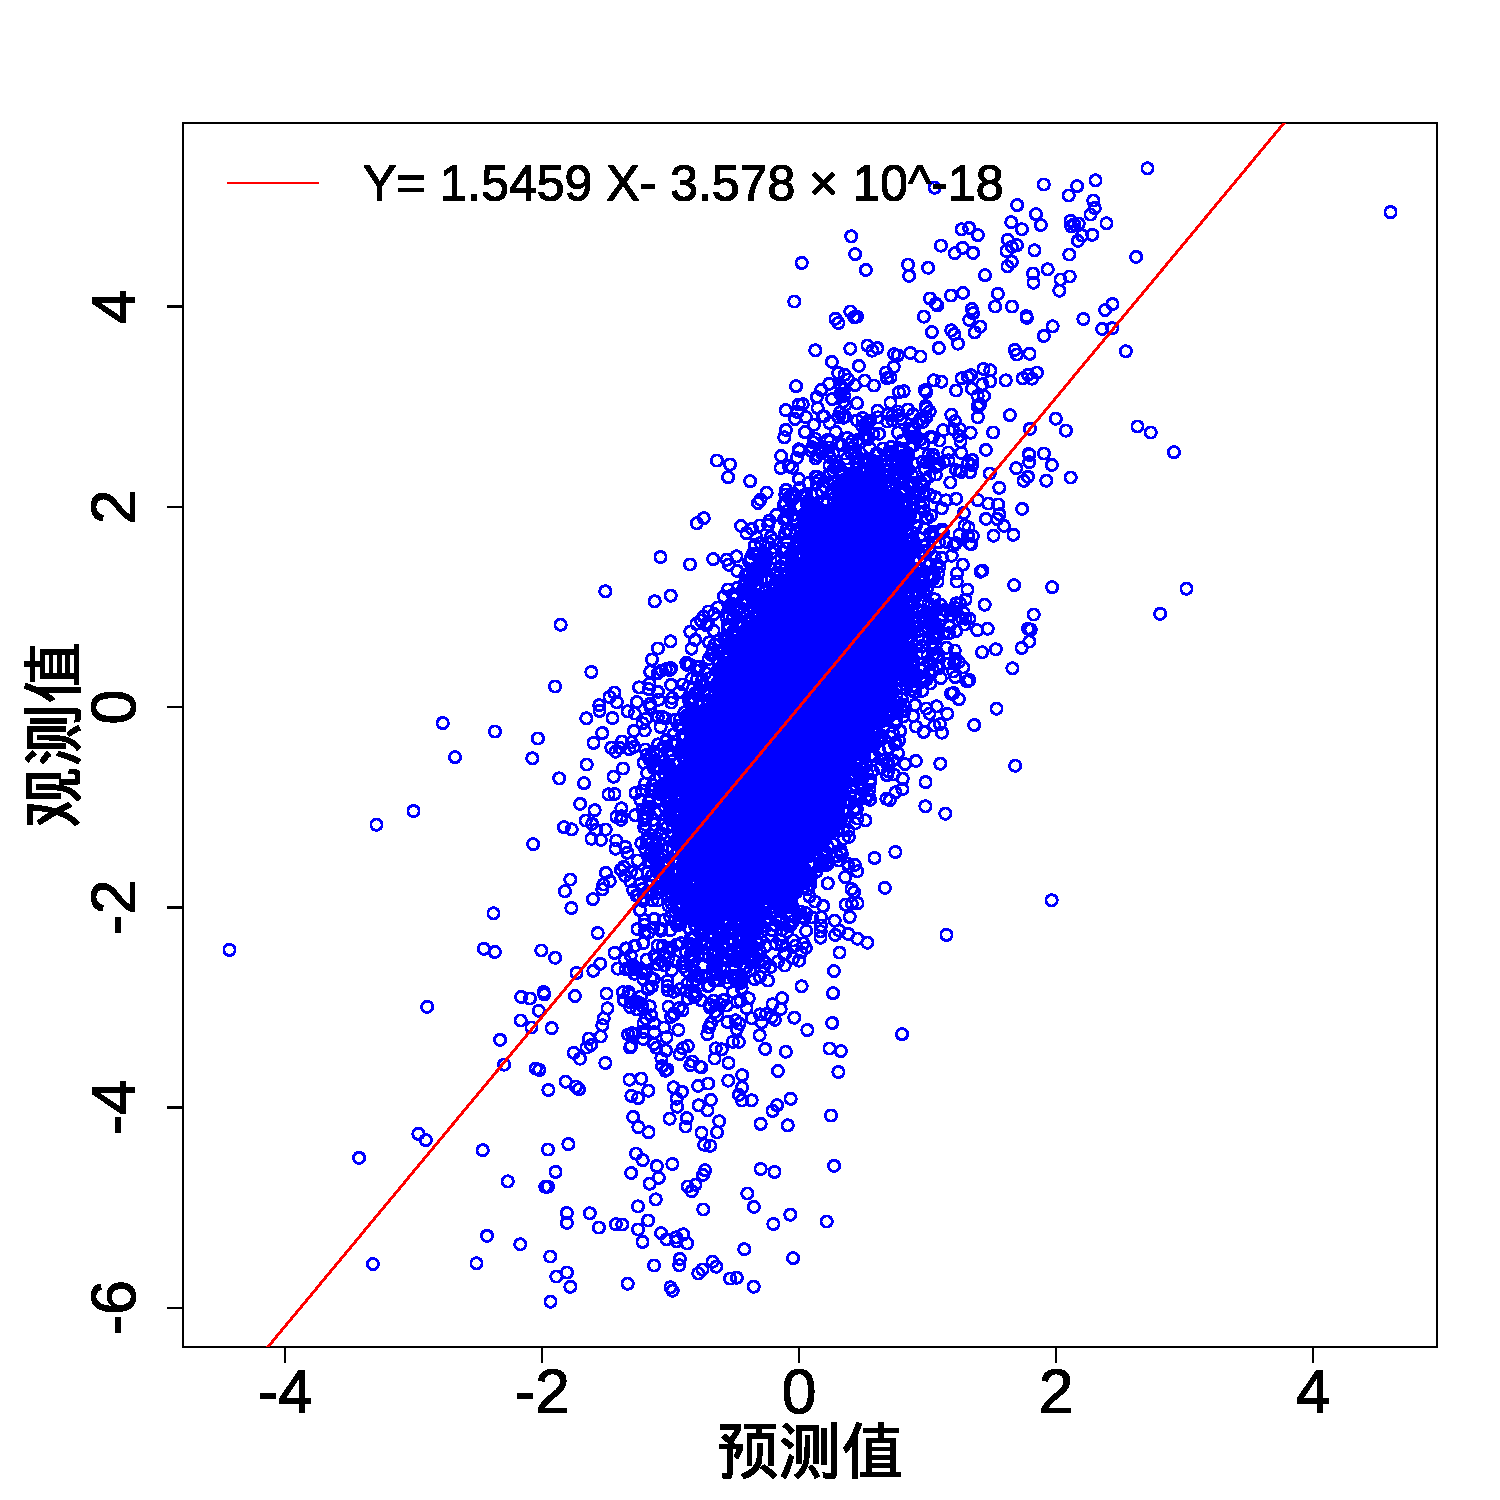
\includegraphics[width=\textwidth]{figures/p_a_scatter_m.pdf}
    \caption{O'Neil数据集的\\预测值和测试值的散点图\label{fig:mc}}
  \end{minipage}
  \begin{minipage}{0.45\linewidth}
    \centering
    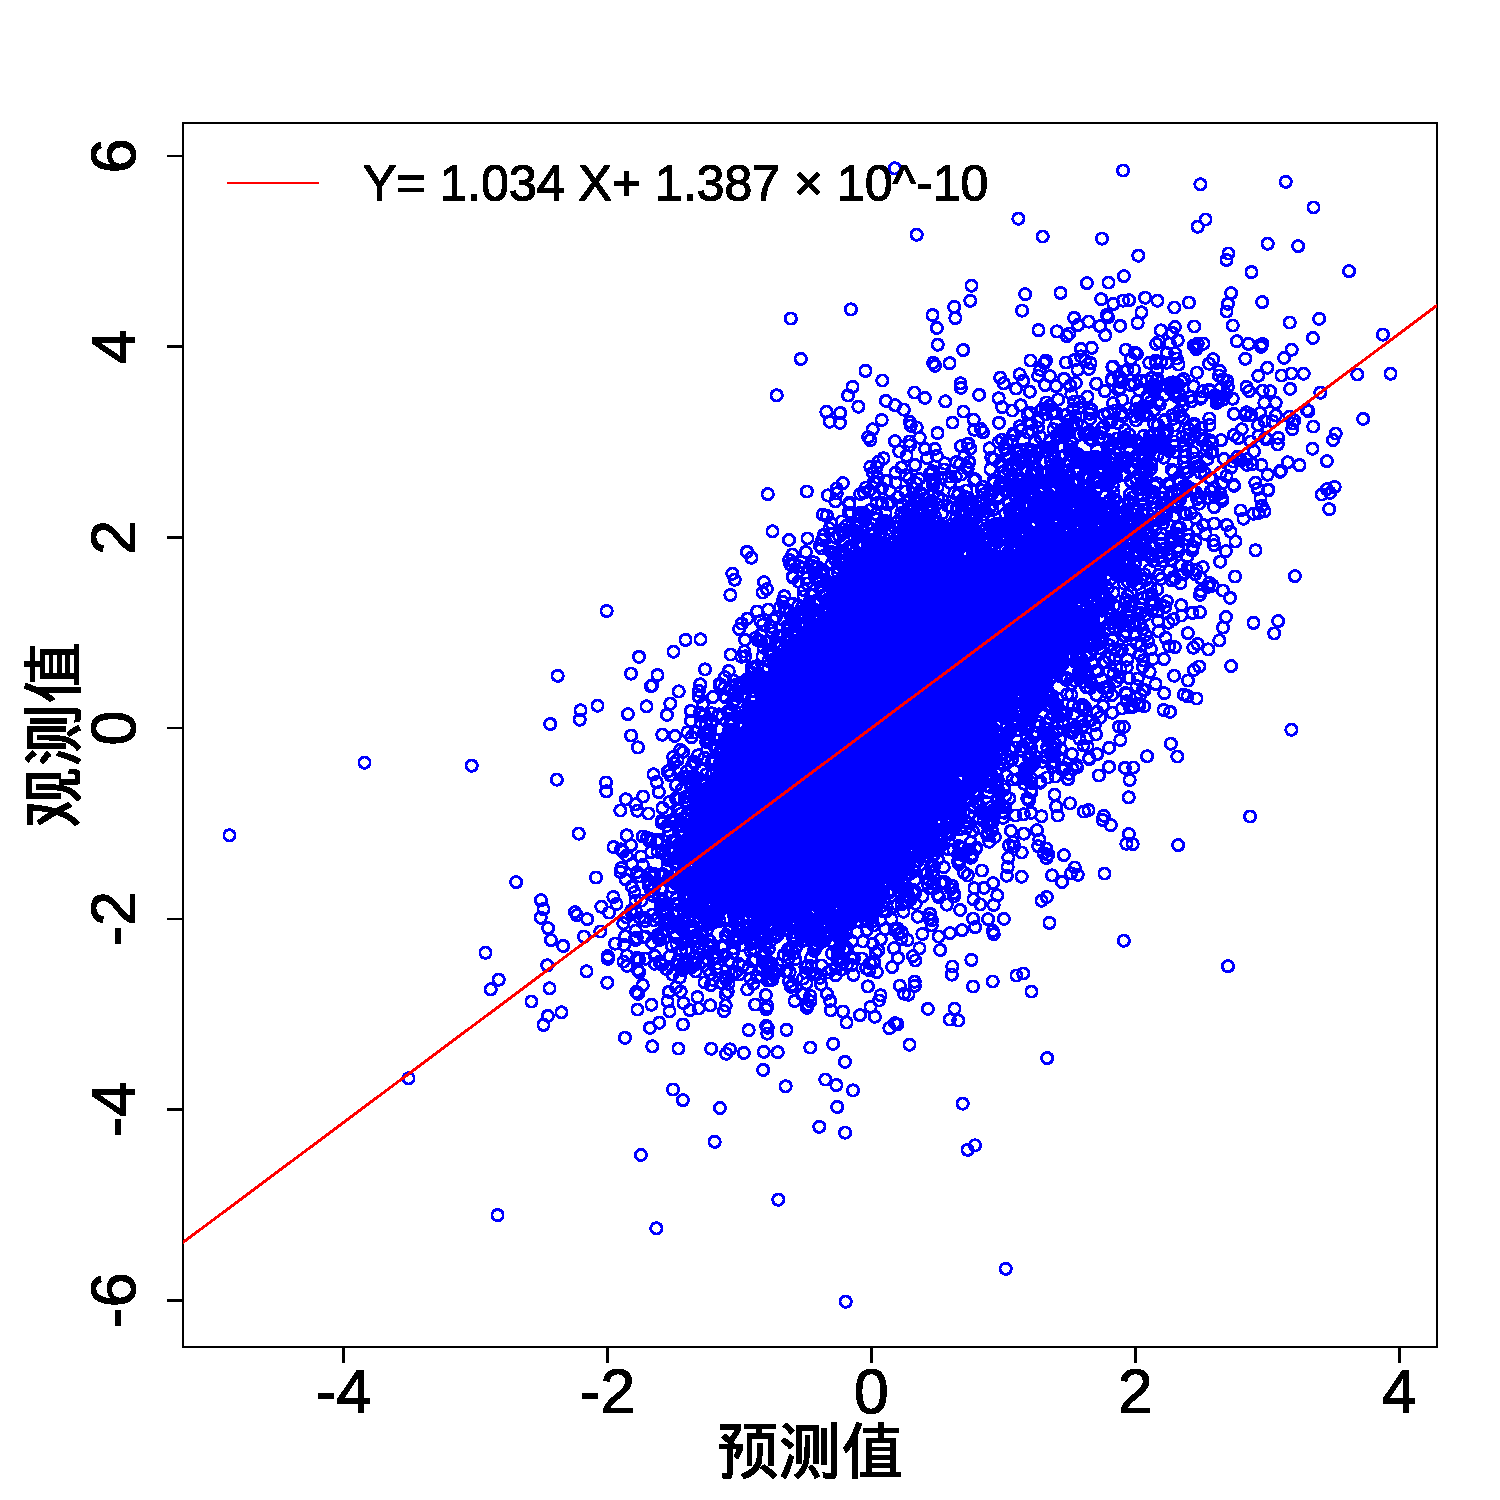
\includegraphics[width=\textwidth]{figures/p_a_scatter.pdf}
    \caption{NCI-ALMANAC数据集的\\预测值和测试值的散点图\label{fig:nc}}
  \end{minipage}
\end{figure}

无论是基于O'Neil数据集还是NCI-ALMANAC数据集,DCSN模型预测结果的拟合函数都表明,DCSN的预测结果和实际测试值之间具有很强的线性相关性。因此,可以得出结论,DCSN模型是一个有效的预测模型,可以用于生物医学领域中的药物组合筛选和发现。

为了统计数据集预测结果中每个药物组合的邻居数情况,本文制作了药物组合邻居数的柱状图,如图\ref{fig:md}和图\ref{fig:nd}所示。其中,可以看到O'Neil数据集中大部分药物组合的高相似邻居数集中在150以前,NCI-ALMANAC数据集中大部分药物组合的高相似邻居数集中在100以前,这说明这些数据集中的药物组合之间的化学结构相似度程度存在差异。

\begin{figure}[H]
\centering
  \begin{minipage}{0.45\linewidth}
    \centering
    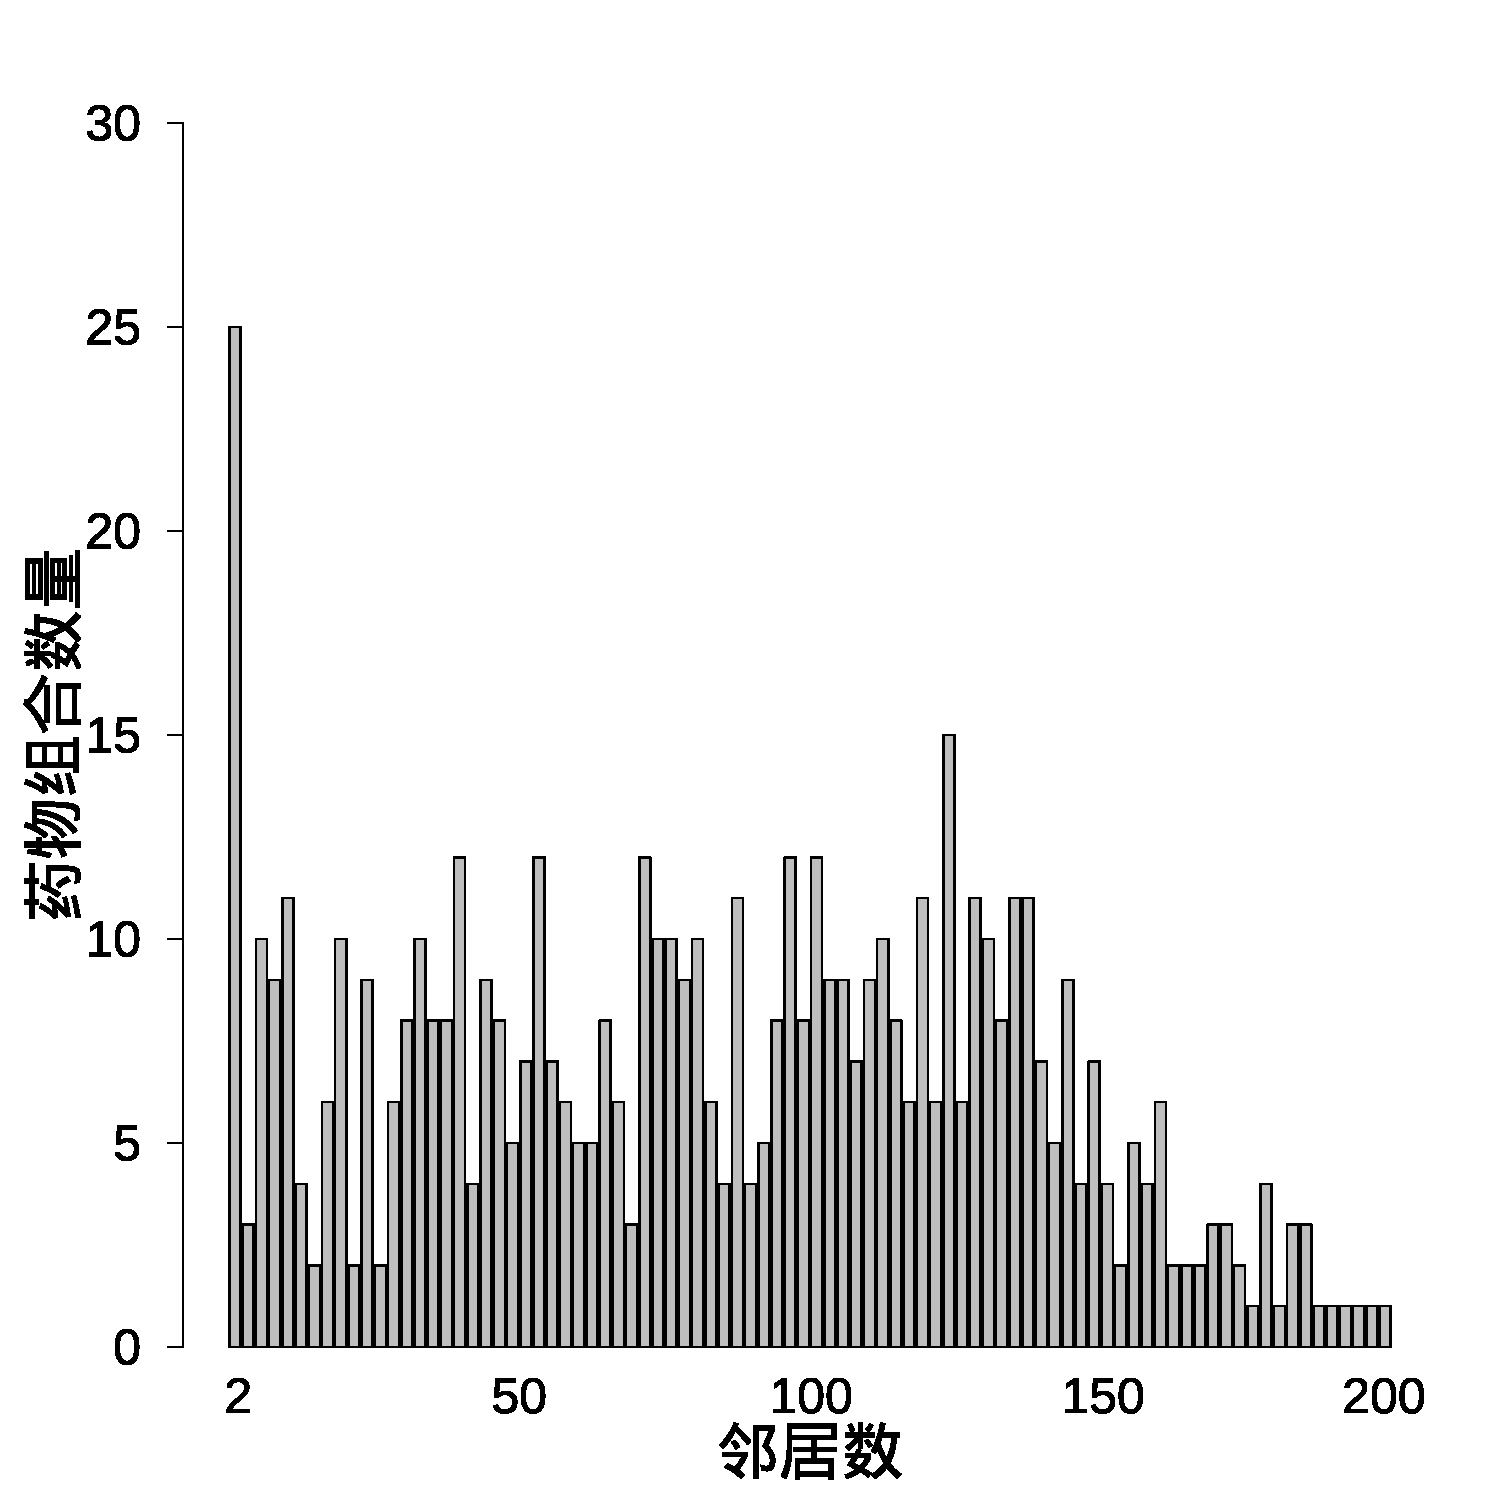
\includegraphics[width=\textwidth]{figures/m_barplot.pdf}
    \caption{基于O'Neil数据集的\\药物组合邻居数柱状图\label{fig:md}}
  \end{minipage}
  \begin{minipage}{0.45\linewidth}
    \centering
    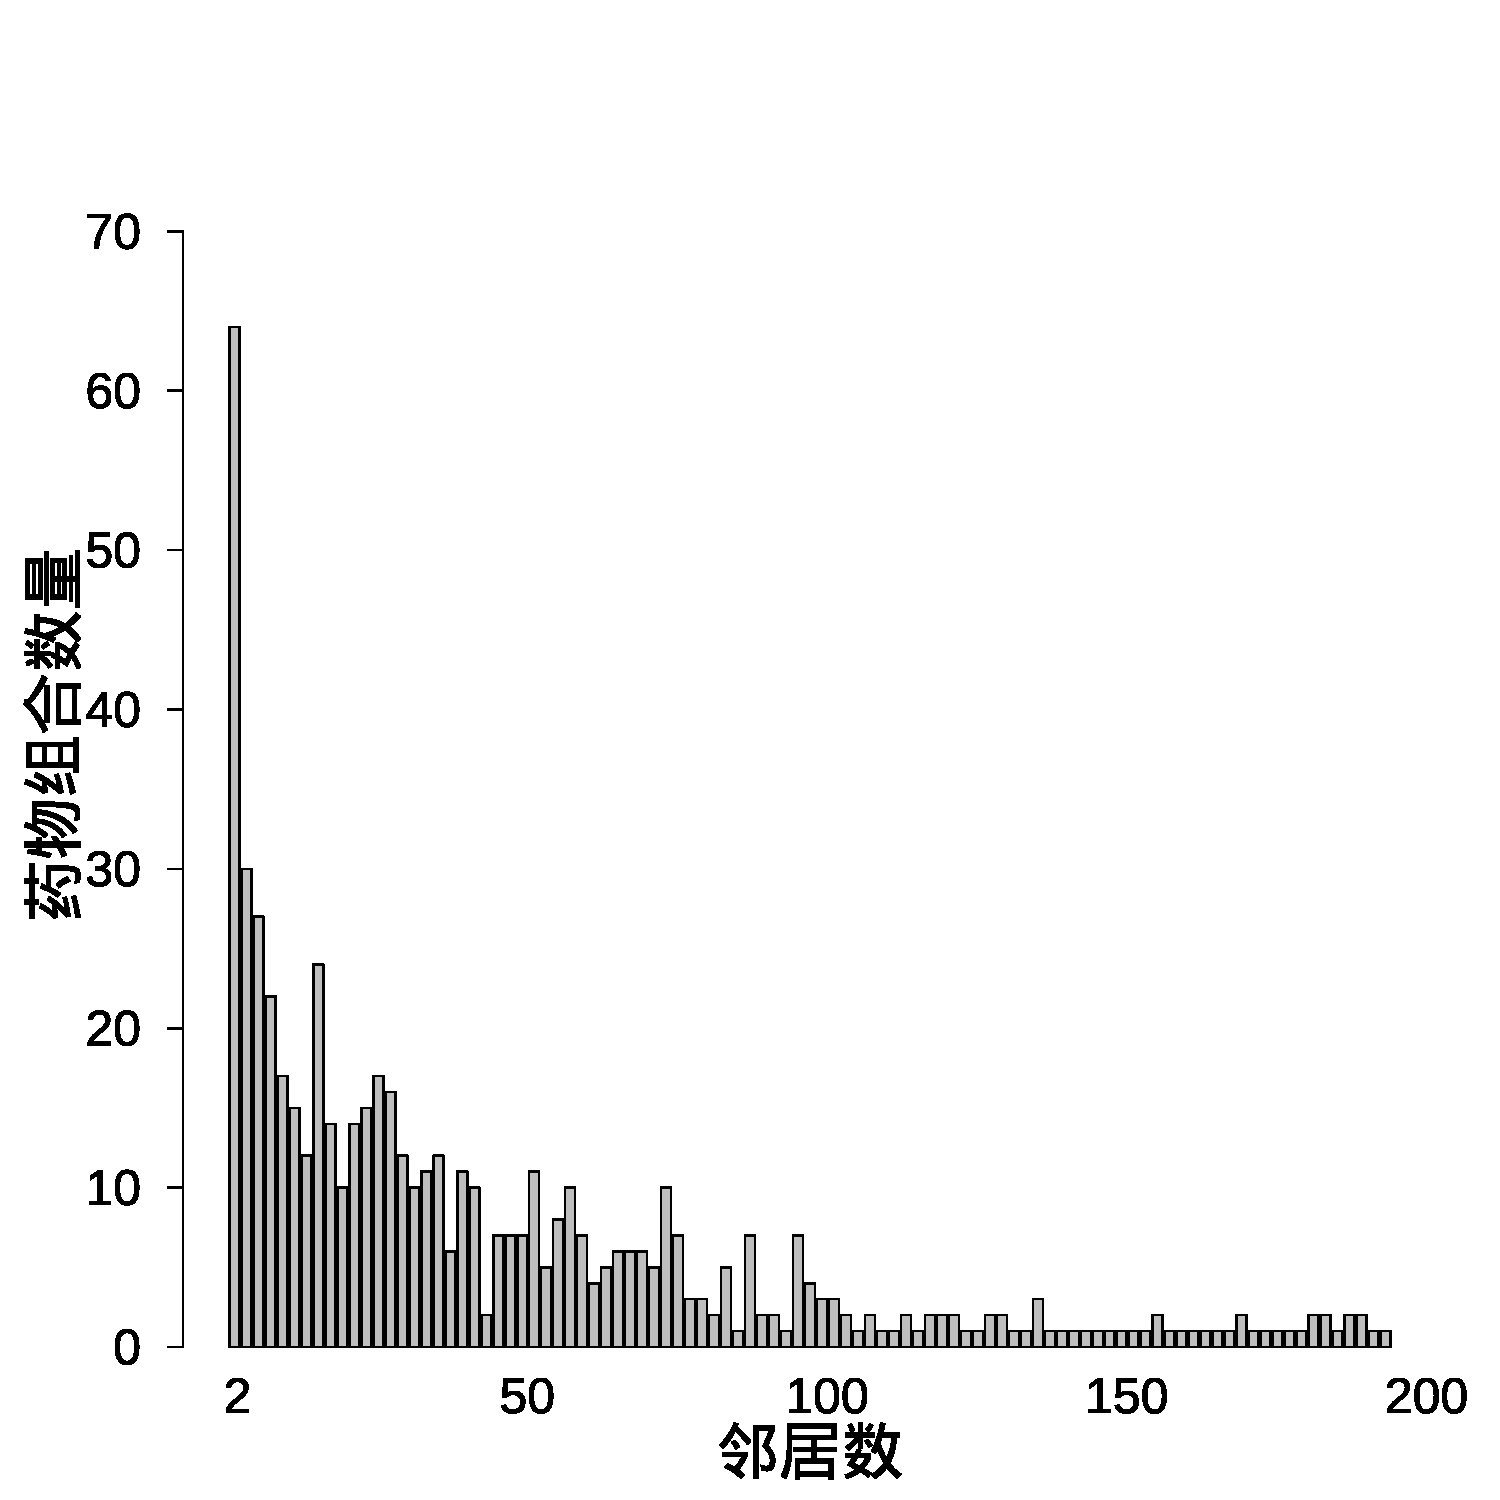
\includegraphics[width=\textwidth]{figures/n_barplot.pdf}
    \caption{基于NCI-ALMANAC数据集的\\药物组合邻居数柱状图\label{fig:nd}}
  \end{minipage}
\end{figure}

\newpage

\begin{figure}[H]
\centering
  \begin{minipage}{0.45\linewidth}
    \centering
    \includegraphics[width=\textwidth]{figures/heatmap_m}
    \caption{基于O'Neil数据集的\\药物组合相似性热图\label{fig:mht}}
  \end{minipage}
  \begin{minipage}{0.45\linewidth}
    \centering
    \includegraphics[width=\textwidth]{figures/heatmap_n}
    \caption{基于NCI-ALMANAC数据集的\\药物组合相似性热图\label{fig:nht}}
  \end{minipage}
\end{figure}

为了探索数据集中的药物组合之间的化学结构相似度的差异程度,本文制作了药物组合相似性热图如图\ref{fig:mht}和图\ref{fig:nht}所示。可以发现后者的红色部分明显比前者多。这一现象说明NCI-ALMANAC数据集中的药物组合之间的化学结构相似度更高,因此使用相对较少的高相似邻居数就足以提供有用的信息,而O'Neil数据集中的药物组合之间的化学结构相似度相对较低,需要使用更多的高相似邻居才能提供有用的信息。这一差异可能是由于两个数据集所包含的化合物种类、药物结构的多样性以及化学数据的采集和处理方法等因素不同所导致的。但是无论在哪个数据集上,大多数药物都能通过使用较少高相似的药物组合进行平移,即可获得与使用目标药物组合相似的效果。这表明,利用高相似邻居药物组合们进行目标药物组合的预测是可行的。

\begin{figure}[htbp!]
\centering
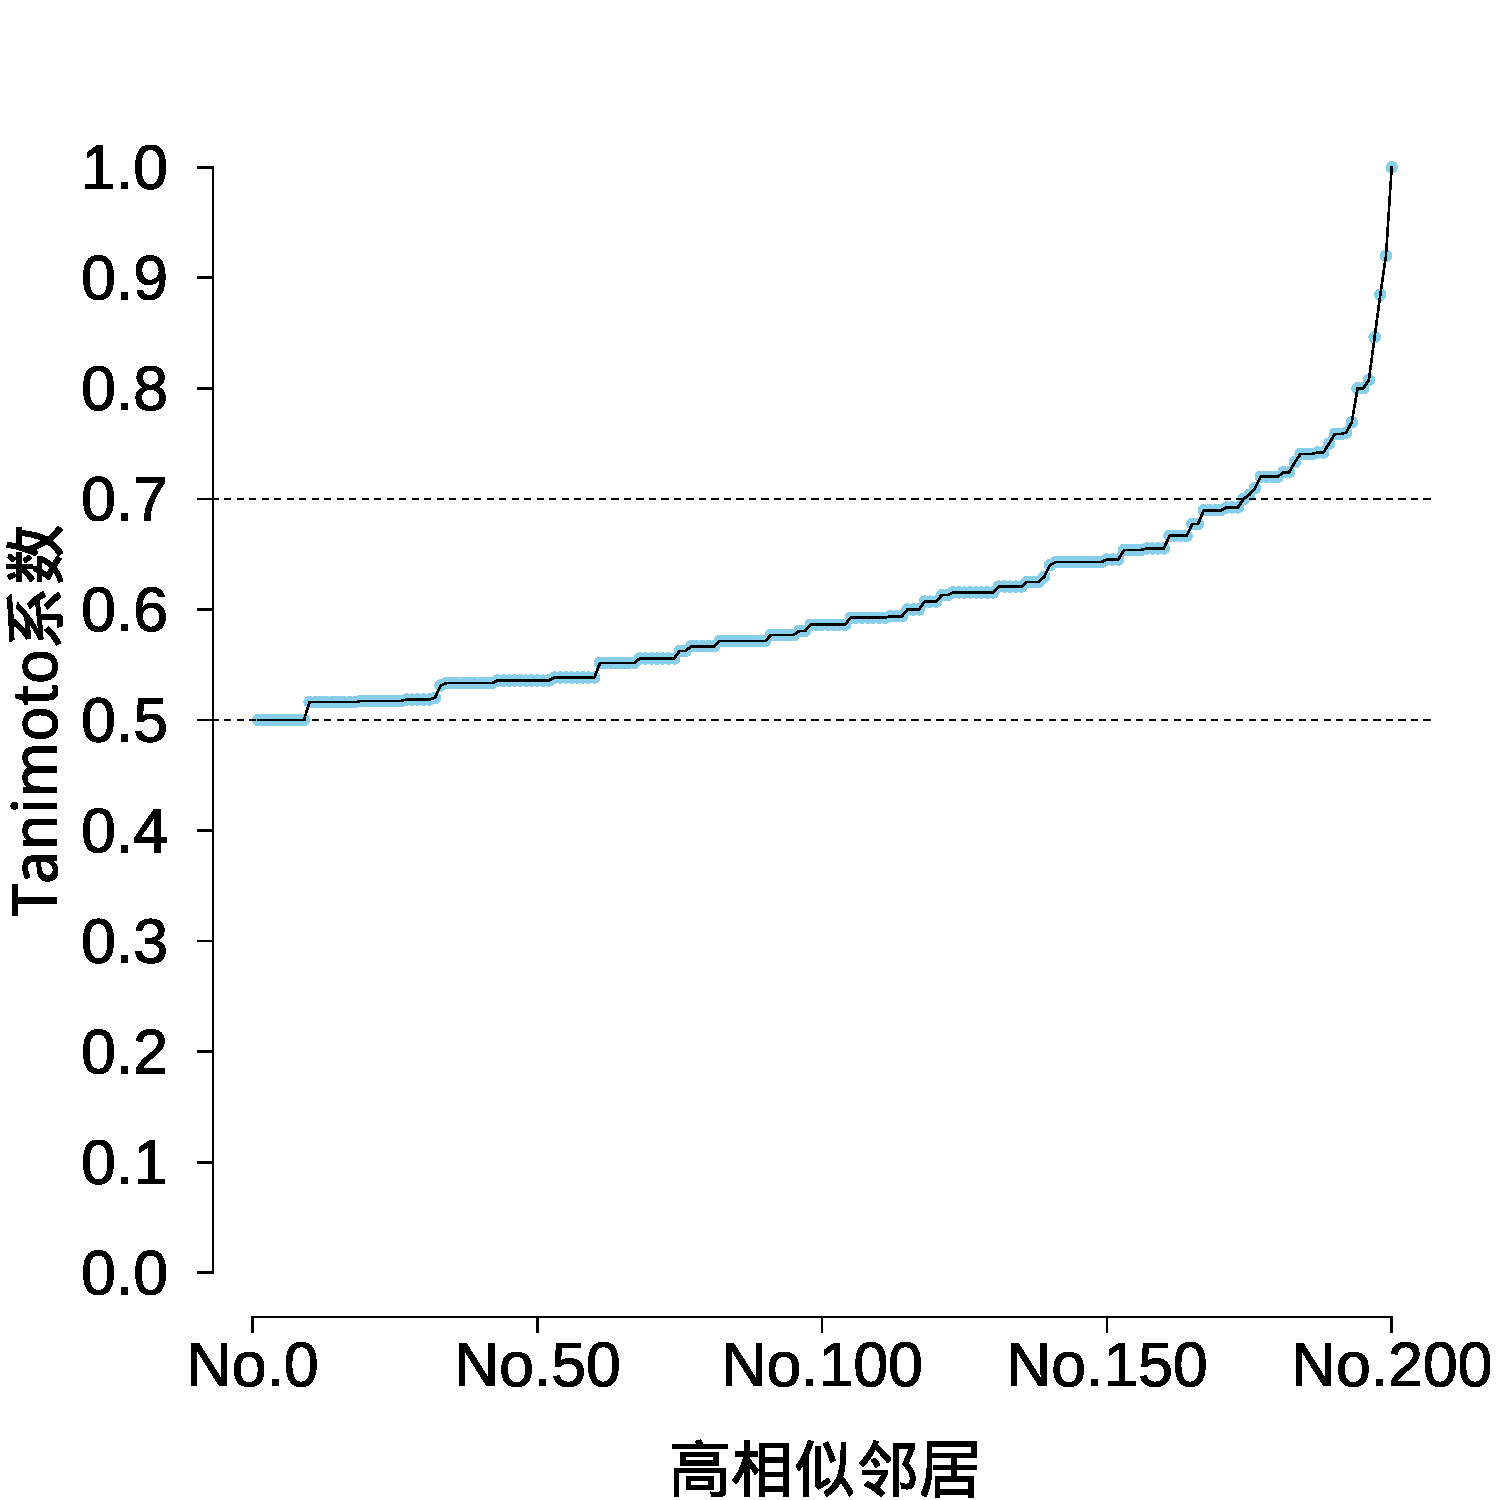
\includegraphics[width=0.5\textwidth]{figures/n_exp.pdf}
\caption{药物组合'Vinblastine sulfate', 'Melphalan'的\\高相似邻居Tanimoto系数图\label{fig:nco}}
\end{figure}

通过对预测结果的观察,在这些药物组合中,可以观察到有一些药物组合的高相似邻居数过多。比如,在NCI-ALMANAC数据集中,有一组药物组合的邻居数最多,它们是'Vinblastine sulfate'和'Melphalan',这组药物组合的邻居数达到了模型求解区间约束的200个邻居。查看它们对应邻居药物组合的Tanimoto系数,从小到大依次排列,如图\ref{fig:nco}所示。可以观察到这200个高相似的邻居中,序号$\mathrm{No.0}$到序号$\mathrm{No.150}$之间药物组合和目标药物组合的Tanimoto相关系数介于0.5到0.7。这表明它们之间具有一定的相关性,但也意味着需要更多相似度更高的药物组合来与目标药物组合匹配,以实现相似的疗效。然而,在实际应用中,这种匹配方法可能会带来问题。治疗方案需要考虑多方面的因素,包括药物之间的相互作用和可能的副作用、患者的个体差异和药物代谢情况等。因此,药物治疗并不可能使用过多的药物组合来治疗病患。如果使用过多的药物组合可能会导致药物相互作用的增加、副作用的加重,并可能会影响药物的疗效。因此,在药物组合治疗中,需要谨慎选择药物组合的数量,以实现最佳的治疗效果。

%插入最少邻居数的图

\section{相关模型的预测结果比较与分析}

本文在横向对比其他模型时,仅采用PCC作为模型的评价指标。这是因为在模型构建前,对数据进行了预处理,这个过程中对原始数据进行了Z-score行标准化,以减少极端值对权重的影响。因此,使用MSE和RMSE等指标进行评估时,DCSN模型与其他使用原始数据的模型相比,结果表现存在超过百倍的差距。在这种情况下,这些指标已失去了比较的价值。因此,本文将重点关注PCC指标来评价模型的表现。

在O'Neil数据集上,本文使用文献\cite{13}中相关的DL模型和ML模型进行比较:深度神经网络(DNN)、梯度提升机(GBM)、随机森林(RF)和支持向量机(SVM),如表\ref{table:model-evaluation}。

\begin{table}[htbp]
  \centering
  \caption{同文献\cite{13}中的模型比较}
  \label{table:model-evaluation}
  \small
  \begin{tabular}{p{4cm}cc}
    \toprule
    Model & PCC & RMSE \\
    \midrule
    DNN & 0.73 & 15.91 \\
    GBM & 0.69 & 16.54 \\
    DCSN & 0.675 & - \\
    RF & 0.65 & 17.49 \\
    SVM & 0.50 & 19.92 \\
    \bottomrule
  \end{tabular}
\end{table}

同时,在NCI-ALMANAC数据集上,本文使用文献\cite{18}中基于高阶分解机(FM)的一阶(comboFM-1)、二阶(comboFM-2),五阶(comboFM-5)模型和随机森林(RF)进行比较,如表\ref{table:sl-evaluation}。

\begin{table}[htbp]
  \centering
  \caption{同文献\cite{18}的模型比较}
  \label{table:sl-evaluation}
  \small
  \begin{tabular}{p{4cm}cc}
    \toprule
    模型 & PCC & RMSE \\
    \midrule
    DCSN & 0.684 & - \\
    comboFM-5 & 0.680 & 62.850 \\
    comboFM-2 & 0.480 & 83.908 \\
    comboFM-1 & -0.156 & 146.672 \\
    RF & 0.41 & 81.27 \\
    \bottomrule
  \end{tabular}
\end{table}

通过比较分析可知,深度学习方法相比于经典机器学习方法,具有更高的PCC,因此具有更优异的效果。而本文所提出的DCSN模型,在PCC方面虽略优于一些机器学习方法,但与深度学习方法相比仍存在较大差距。不过,从实际应用角度考虑,本文的DCSN模型所需的硬件资源较少,最优求解方法仅使用32核CPU运行6个小时即可得出结果。相比较而言,深度学习方法需要依赖显卡进行计算,所需的硬件资源较多,且耗费时间更长。因此,本文所提出的模型具有较低的复杂度,更适合于初期药物筛选阶段的抗癌药物组合协同作用研究,并更利于早期研究的进行。

\section{本章小结}

本章介绍了模型评价与比较的结果。首先,使用PCC和RMSE作为评价指标,评估了四种模型求解方法,发现精细调参法在准确性方面表现最佳,具备强大的泛化能力和预测性能。此外,绘制了协同得分预测值和测试值的散点图,并使用最小二乘回归法对数据进行拟合,结果显示回归系数显著。制作了药物组合邻居数的柱状图和散点图,观察到尽管部分药物组合的高相似邻居选取过多,但大多数药物组合的高相似邻居数较少,具有实际应用意义。最后,对比了其他模型的预测性能,以PCC作为评价指标,尽管与大多数DL模型仍有差距,但DCSN模型的复杂度较低,需要的硬件资源更少,时间成本更低。
  % \include{chapter/chap-5}
%  \include{chapter/chap-6}
%  \include{chapter/chap-7}
  % !Mode:: "TeX:UTF-8"
\begin{conclusion}
\label{chap:conclusion}

本文聚焦抗癌药物组合协同作用预测问题,构建了形式简单、直观易懂的药物组合相似性网络模型DCSN,并将其应用于两大抗癌药物组合高通量筛选数据集,O'Neil 数据集和 NCI-ALMANAC 数据集,得到的具体结论如下: 

(1) 提出了药物组合相似性假设:分子指纹相似的药物组合对于固定细胞系具有相似的协同作用。该假设反映了药物组合分子指纹之间的相似度与其协同得分之间的关系,并且通过如下实验现象得到了验证:高相似药物组合团的协同得分相关性较强,低相似药物组合团的协同得分相关性较弱。 

(2) DCSN在O'Neil 数据集和 NCI-ALMANAC 数据集上都取得了较为理想的预测结果,预测协同得分与观测协同得分的PCC分别为0.675和0.684,优于部分经典的机器学习模型,但低于深度学习模型DNN。特别值得一提的是,DCSN仅涉及两个参数,分别是邻居数和衰减率,模型的计算成本极低。结果表明:DCSN可以作为新药物组合高通量虚拟筛选的可选择工具。 

尽管本文的研究工作取得了一些成果,但仍有改进的空间。后续进一步研究的问题如下:

(1) 在相似性分析中,除了本文采用的 Tanimoto 系数和 Spearman 相关系数,还可以考虑使用其他距离度量方法,以提高相似性分析的准确度。

(2) 可以将药物靶向信息、联合用药信息、细胞系的基因表达信息、基因组突变信息和拷贝数变异信息整合到模型中,提高药物组合协同作用预测的精度。

(3) 可以通过设定邻居数阈值来优化筛选和预测药物协同作用得分的方法。这样,即使某些药物没有高相似邻居,仍能进行筛选和预测,避免某种药物具有过多高相似邻居的情况,确保筛选方法具有实际应用意义。

(4) 基于本文相同的理念,未来可以考虑验证“相似的细胞系对于固定药物组 合具有相似的协同作用”这一假设,进而构建细胞系相似性网络模型,实现新细胞系的抗癌药物组合协同作用预测。

\end{conclusion}

  %% 附录
  % \appendix
  % \include{chapter/appendix}


% 以下为附件部分
%----------------------------%
\backmatter

  % 参考文献
  \bibliography{bib/tex}
  %\include{chapter/bib}


  % 致谢
  % !Mode:: "TeX:UTF-8"
\begin{thanks}

在导师   老师的亲切关怀和悉心指导下,本研究得以顺利完成。在过去的两年多时间里,李老师不仅在学术上给予我细致入微的指导,也在生活上给予了特别的关心,为我提供了良好的学习和科研条件。从课题学习到论文选题,再到课题立项、论证、研究、实验、总结、论文撰写和修订,每个环节都蕴含着导师的心血和付出。李老师渊博的知识、严谨的治学态度以及高尚的品质使我受益匪浅,她不仅是我科研工作的启蒙者和指引者,更是我生活和做人的楷模。值此论文完成之际,我谨向导师表达最崇高的敬意!

此外,我还要衷心感谢燕山大学理学院的老师、同学和朋友,他们在我学习和生活上给予了无私的帮助。感谢学校为我们提供了良好的学习环境和丰富的图书馆资源!同时,我要特别感谢我的父母,在他们的大力支持下,我才得以顺利完成学业!他们的支持与鼓励是我前进的动力。再次向所有关心、支持和帮助过我的人表示衷心的感谢!

\end{thanks}



\end{document}
